\chapter{Proposal for a new \textit{\textit{Naldaviricetes}} viral family associated with Hymenoptera parasitoids}
    \label{chap:LbFV-Family-description}
    
        \begin{center}
        \Large Benjamin Guinet$^{\text{1}}$$^{\text{*}}$, Matthieu Leobold$^{\text{2}}$$^{\text{*}}$, Nelly Burlet$^{\text{1}}$, Jean-Michel Drezen$^{\text{2}}$, Elisabeth Herniou$^{\text{2}}$, Annie Bézier$^{\text{2}}$$^{\text{*}}$, Julien Varaldi$^{\text{1}}$$^{\text{*}}$\\
        \vspace{0.5cm}
        \normalsize
        $^{\text{1}}${Université Lyon 1, CNRS, Laboratoire de Biométrie et Biologie Evolutive UMR 5558, F-69622 Villeurbanne, France.}\\
        $^{\text{2}}${Institut de recherche sur la biologie de l'insecte UMR7261 Université de Tours, Centre National de la Recherche Scientifique : UMR7261 Av Monge 37200 Tours, France.}\\
        $^{\text{*}}${Co-first and co-last authors.}\\
    \end{center}
     \setcounter{minitocdepth}{1}

    {\hypersetup{linkcolor=GREYDARK}\minitoc}

\clearpage

\label{sec:chap2}

\section{Reproducibility and Supplemental material}

All supplementary material named with a "GitHub" mark, can be found within the following GitHub repository : \href{https://github.com/BenjaminGuinet/PhD_defense/tree/main/Supplementary_paper2}{Supplementary\_paper2}. An e-mail authorization must have been sent to all members of the jury.

\section{Abstract}

Large dsDNA viruses from the \textit{Naldaviricetes} class are currently composed of four viral families infecting insects and/or crustaceans. Since the 1970s, particles described as filamentous viruses have been observed by electronic microscopy in several species of Hymenoptera parasitoids but until recently no genomic data was available. This study provides the first comparative genomic analyses of these filamentous viruses. We studied the genomes of seven filamentous viruses, six of which were newly obtained, in addition to the previously sequenced Leptopilina boulardi filamentous virus (LbFV), to gain a better understanding of their evolutionary history. We show that filamentous viruses related to LbFV share morphological, genomic and phylogenetic features that distinguish them from their closest relatives, i.e. \textit{Hytrosaviridae}. Additionally, these filamentous viruses share all genomic features of the \textit{Naldaviricetes} but their core genome comprises five specific genes that clearly distinguish them from Hytrosaviruses. Furthermore, by mining public databases, we provide evidence suggesting they preferentially infect Hymenoptera with parasitoid lifestyle. Finally, we propose a taxonomical revision of the class \textit{Naldaviricetes} in which filamentous viruses related to LbFV constitute a fifth family within the order \textit{Lefavirales}. We propose to name this new family, Filamentoviridae. 

\section{Introduction}

All cellular life forms are associated with viruses \citep{kristensen_new_2010,koonin_virocentric_2013}. However, rough but reasonable estimations of viral diversity suggest that only 1\% of all eukaryotic viruses has been discovered and classified \citep{geoghegan_comparative_2017}. Because arthropods are the most diverse taxonomic group of animals, we may expect that a great fraction of this unknown viral diversity is hosted by arthropods. Indeed, our assessment of arthropod viral diversity has recently been progressing thanks to the development of high-throughput sequencing technologies. These technologies permitted deep (possibly meta-) genomic and transcriptomic analysis that uncovered part of this unknown diversity \citep{ dolja_metagenomics_2018,roux_diversity_2022, wu_abundant_2020,schulz_giant_2020}. For RNA viruses, the discovery of new lineages is facilitated by presence of the universal RNA-dependent-RNA polymerase. By screening RNAseq datasets, it has been possible to identify tens or thousands of new viruses in single large-scale bioinformatic analysis \citep{shi_evolutionary_2018, wu_abundant_2020, medd_virome_2018,obbard_new_2020}. On the contrary, DNA viruses do not share any universal genes \citep{koonin_global_2020} and are prone to extensive gene loss, gain, and exchange. These features thus make exploration of the "DNA virosphere" more challenging.  

Among eukaryotic large dsDNA viruses, the \textit{Naldaviricetes} forms a monophyletic class of arthropod-infecting viruses with specific features. These viruses have circular genomes replicating in the nucleus and packaged into enveloped rod-shaped nucleocapsids. They belong to four families: the \textit{Baculoviridae}, \textit{Nudiviridae}, \textit{Hytrosaviridae}, and \textit{Nimaviridae} \citep{harrison_ictv_2020}. They share a group of genes that encode the so-called \textit{per os} infectivity factors (PIFs). PIFs are required for baculovirus entry into midgut goblet cells during primary infection (Rohrmann, 2019) and they may be involved in particle entry into other cell types, i.e., salivary glands for hytrosaviruses \citep{abd-alla_genome_2008,garcia-maruniak_sequence_2008}, gonad cells for Helicoverpa zea nudivirus 2 \citep{hamm_oviposition_1996,burand_analysis_2012} and all cell types of the parasitized Lepidoptera for bracoviruses (endogenous nudiviruses found in some parasitic wasps) \citep{bezier_polydnaviruses_2009, muller_genome-wide_2021}. Among \textit{Naldaviricetes}, the \textit{Baculoviridae}, the \textit{Nudiviridae}, and the \textit{Hytrosaviridae} form the order \textit{Lefavirales}. This name derives from the fact that they share the so-called \textit{lef} genes (for late expression factor) encoding the different subunits of a specific viral \textit{RNA polymerase}. These \textit{lef} genes ensure transcription of viral genes in the late phase of infection. 

Since the 1970s, investigations using electron microscopy uncovered a variety of viruses in the reproductive tract of Hymenopteran parasitic wasps. In particular, several endoparasitoid wasp species were found to harbor long flexible rod-shaped enveloped particles replicating in their ovaries. These particles are often secreted in the genital fluid, which is injected during wasp oviposition into the parasitized host. Because of the peculiar shape of these particles, the viruses were referred to as "filamentous viruses" (FVs). Such FVs were described in different species: a Campopleginae (\textit{Diadegma terebrans}), a series of Braconidae (\textit{Cotesia congregata}, \textit{Cotesia hyphantriae}, \textit{Cotesia marginiventris}, \textit{Microplitis croceipes} and \textit{Microplitis rufiventris}) and a Figitidae (\textit{Leptopilina boulardi}) \citep{krell_replication_1987, de_buron_characterization_1992,  stoltz_viruses_1979, hamm_comparative_1990,hegazi_calyx_2005, varaldi_infectious_2003,varaldi_artifical_2006}.

More recently, a first "filamentous virus" was characterized at the molecular level from the \textit{Drosophila} parasitoid \textit{Leptopilina boulardi} \citep{lepetit_genome_2017}. This virus was named Leptopilina boulardi filamentous virus (LbFV) and phylogenetic analysis clearly identified it as a sister group of hytrosaviruses, known to induce salivary gland hypertrophy symptoms in dipteran adults \citep{abd-alla_hytrosaviridae_2009}. However, it has been suggested that this virus may belong to a new family based on its high sequence divergence from \textit{Hytrosaviridae} \citep{lepetit_genome_2017}. Interestingly, LbFV has a strong impact on the wasp egg-laying behavior: infected females readily accept to lay their eggs in already parasitized hosts, contrary to uninfected ones \citep{varaldi_infectious_2003,varaldi_artifical_2006}. This induction of "superparasitism" permits virus horizontal transmission, thus increasing its fitness at the expense of wasp fitness \citep{gandon_superparasitism_2006}. Furthermore, an ancestral integration of a related virus has been described in \textit{Leptopilina} species (Di Giovanni et al., 2020). Similarly to other parasitoid wasp species that have domesticated viruses \citep{bezier_polydnaviruses_2009,volkoff_analysis_2010,pichon_recurrent_2015, burke_common_2019}, these endogenized viral genes have been domesticated and are employed by female wasps as a means of delivering virulence factors, which are necessary to protect their eggs from the host immune system \citep{rizki_parasitoid_1990, di_giovanni_behavior-manipulating_2020}. Recently, sequences of a virus related to LbFV were detected in a sample of field-collected \textit{Drosophila melanogaster} (DmFV) \citep{wallace_discovery_2021}. Given the potential high prevalence of \textit{Leptopilina} parasitoids in the field \citep{patot_prevalence_2010}, it is unclear whether this virus was really infecting \textit{Drosophila} cells or whether it was introduced into the \textit{Drosophila} by an infected parasitic wasp during an unsuccessful parasitization event. Another type of distantly related filamentous virus is known to infect \textit{Apis mellifera} (AmFV). Also belonging to the \textit{Naldaviricetes}, this virus however lacks genomic characteristics from the \textit{Lefavirales} \citep{gauthier_apis_2015, yang_genomics_2022}. 

In this study, we characterize six new virus genomes related to LbFV, infecting wasps that belong to three Hymenoptera superfamilies (Cynipoidea, Chalcidoidea and Ichneumonoidea). By in-depth comparative genomic and phylogenomics of their genomes together with particle morphogenesis comparison, we explore the possibility that these "filamentous viruses" constitute a new viral family within \textit{Naldaviricetes}. We show that these filamentous viruses share morphological, genomic and phylogenetic features that distinguish them from their closest relatives, i.e. \textit{Hytrosaviridae}. Additionally, by mining public databases, we provide evidence suggesting that filamentous viruses preferentialy infect Hymenoptera with parasitoid lifestyle.  We therefore propose a taxonomical revision of the class \textit{Naldaviricetes} in which filamentous viruses related to LbFV do not belong to \textit{Hytrosaviridae} but constitute a fifth family within the order \textit{Lefavirales}. We propose to name this new family Filamentoviridae. 

\section{Results}

\subsection{Genomes of filamentous viruses related to LbFV have similar structures}   

We analyzed the genome sequence of six novel viruses related to the Leptopilina boulardi filamentous virus (LbFV). All of them were obtained from parasitoid wasps, namely \textit{Leptopilina heterotoma} (Cynipoidea, Figitidae), \textit{Encarsia formosa} (Chalcidoidea, Aphelinidae), \textit{Platygaster orseoliae} (Platygastroidea, Platygastridae), \textit{Psyttalia concolor} (Ichneumonoidea, Braconidae) and two \textit{Cotesia congregata} incipient species (Ichneumonoidea, Braconidae). One viral sequence was retrieved following particle purification while the other five were discovered after genome sequencing of parasitoid wasps (\figurename{\ref{figure:Table_genomes_filamentous}}). In the following, the viruses are referred to as the two initials of the binomial latin name of the wasp followed by FV for filamentous virus (i.e.: LhFV, EfFV, PoFV, PcFV, CcFV1 and CcFV2, respectively).  

In the five datasets obtained from parasitoid whole genome sequencing projects, we had to ensure that the putative viral contigs were not endogenized in wasp chromosomes. To do so, we studied the sequencing depth or coverage for each contig. Our expectation was that the coverage should differ between wasp chromosomes and viral chromosomes, since the probability that both entities had the same density in the DNA extract is most likely low. As expected, coverage was significantly different between viral and parasitoid contigs for all five biological models (\figurename{\ref{figure:ALL_filamentous_cov_GC_plot}}), strongly suggesting that viral contigs effectively belong to exogenous viruses. The minimal coverage for the presumably viral contigs was high for four of them (\figurename{\ref{figure:ALL_filamentous_cov_GC_plot}}). The last genome (EfFV) had only an approximate 24x coverage based on short reads. However, the additional long read sequencing that was performed on this genome led to a single circular molecule (\figurename{\ref{figure:CcFV1_CcFV2_EfFV_circos}}), confirming that this was indeed a viral genome. Two other genomes (CcFV1 and CcFV2) were also obtained after long-read or Illumina paired-end sequencing (\figurename{\ref{figure:Table_genomes_filamentous}}), leading to a single circular DNA molecule, strongly suggesting that they were complete (\figurename{\ref{figure:CcFV1_CcFV2_EfFV_circos}}). Even though no circular forms could be obtained for the three other genomes (LhFV, PoFV and PcFV), we consider that the obtained sequences are nearly complete since contig cumulative sizes range from approx 106 to 131 kb which is comparable to those of the four circularized FV genomes: approx 111 kb (LbFV), approx 101 kb (CcFV1), approx 138 kb (CcFV2) and 164 kb (EfFV) (\figurename{\ref{figure:Table_genomes_filamentous}}); and more globally to other \textit{Lefavirales} genomes (\textit{Baculoviridae}: 80-180 kb, \textit{Nudiviridae}: 97-232 kb and \textit{Hytrosaviridae}: 125-191 kb) (GitHub:\href{https://github.com/BenjaminGuinet/PhD_defense/blob/main/Supplementary_paper2/Table%20S2.xlsx}{TabS2}). Of note, LhFV sequences have 97.98\% nucleotidic identity with the recently published sequences annotated as Drosophila-associated filamentous virus (DmFV). Such contigs were indeed detected after mining genomic sequences obtained from 6668 pool-sequenced \textit{Drosophila}, sampled from forty-seven European locations \citep{wallace_discovery_2021}. Among these samples, one single was positive for DmFV. Thus, adding to our results the fact \textit{Leptopilina} species (e.g., \textit{L. boulardi} and \textit{L. heterotoma}) parasitize \textit{Drosophila} larvae \citep{kopelman_immature_1984,schlenke_contrasting_2007}, the authors acknowledged they could not detect any DmFV sequences in \textit{D. melanogaster} public datasets and the virus they sequenced could infect the parasitoid wasp rather than the fly \citep{wallace_discovery_2021}; it is likely that LhFV and DmFV correspond to one single virus infecting a wasp that had previouly parasitized the sequenced \textit{Drosophila}.  

Additionally, de novo gene prediction showed a composition of 110 to 128 ORFs for these three non-circularized genomes, which is comparable to the number of ORFs predicted for the three new circular genomes (CcFV1 = 104, CcFV2 = 112, and EfFV = 156; (\figurename{\ref{figure:Table_genomes_filamentous}}, and GitHub:\href{https://github.com/BenjaminGuinet/PhD_defense/blob/main/Supplementary_paper2/Table%20S3.xlsx}{TabS3}), and more generally to related viruses (LbFV = 108, \textit{Naldaviricetes} = 90-241). The presence of repetitive sequences as previously observed for LbFV \citep{lepetit_genome_2017}, is probably the reason underlying our incapacity to circularize these three genomes using short reads only (\figurename{\ref{figure:Table_genomes_filamentous}}). Finally, all six virus genomes had high gene densities (min = 79.9\% and max = 92\%) as observed for viruses belonging to \textit{Naldaviricetes} (\figurename{\ref{figure:Table_genomes_filamentous}}). Altogether, these data strongly suggest that the six novel viral sequences presented here represent complete circularized or complete non-circularized viral genomes.  

\subsection{The filamentous virus core gene set} 

Viral genomes contain two types of genes. On the one hand, the core genes are defined as the set of genes shared by all members of a virus family and are generally involved in essential functions in the virus cycle. On the other hand, accessory genes may be specific to a clade or to particular viruses, may be involved in adaptation to the host, and sometimes acquired from infected hosts by horizontal gene transfer. Only core genes are relevant for the phylogenetic inference of the virus relationships within the virosphere. 

The analysis of the seven filamentous viruses, excluding the contigs of DmFV \citep{wallace_discovery_2021}, resulted in the identification of a set of 29 core genes (\figurename{\ref{figure:dsDNA_filamentous_heatmap}} and GitHub:\href{https://github.com/BenjaminGuinet/PhD_defense/blob/main/Supplementary_paper2/Table%20S4.xlsx}{TabS4}). About two thirds of the genes are homologs of core genes found in different \textit{Lefavirales} and are involved in specific viral transcription, packaging of the virus DNA in the nucleocapsids, assembly and morphogenesis of the particles or virus entry into infected cells (infectivity) as characterized mainly in baculoviruses (\figurename{\ref{figure:dsDNA_filamentous_heatmap}}, green columns). Eight conserved genes encode proteins with unknown function as no sequence similarity was detected (\figurename{\ref{figure:dsDNA_filamentous_heatmap}}). Among these genes, five were strictly specific to FVs related to LbFV (\figurename{\ref{figure:dsDNA_filamentous_heatmap}}, blue columns). 

 \begin{figure}[!htpbt]
\includegraphics[width=\linewidth,height=\textheight,keepaspectratio]{PhD-master/figures/dsDNA_filamentous_heatmap.pdf}\centering
\caption[Paper2:\textit{Naldaviricetes} core genes heatmap]{\textbf{Heatmap representing the core gene content of LbFV related FVs (LbFV-like) compared to other \textit{Naldaviricetes} dsDNA viral species}. A cladogram phylogeny is reported on the right. The rows represent the viral species, and the columns represent the genes distributed according to their potential functions. Colored cells represent the presence of the gene in viral genomes (pale yellow = core genes shared by \textit{Naldaviricetes} species, green = core genes shared by \textit{Lefavirales} species, red = FV and hytrosavirus core genes, blue = FV core genes and grey = presence in other virus genomes).}
\label{figure:dsDNA_filamentous_heatmap}
\end{figure}

In the section that follows, we will first provide evidence that filamentous viruses related to LbFV (i.e., Filamentoviridae) possess all the necessary genes to be classified as \textit{Naldaviricetes} as well as \textit{Lefavirales} clades. We will then provide information regarding the putative function of some of these filamentous core genes. 

All the core genes shared by the \textit{Naldaviricetes} including the per os infectivity factors (\textit{p74}, \textit{pif-1}, \textit{pif-2}, \textit{pif-3} and \textit{pif-5}), the \textit{DNA polymerase} (\textit{DNApol}) and the sulfhydryloxidase (\textit{p33}) were present in the analyzed FV genomes (\figurename{\ref{figure:dsDNA_filamentous_heatmap}}, pale yellow columns). Five out of the six known \textit{Lefavirales} core genes can also be unambiguously predicted as functional ORFs within these genomes, including three subunits of the RNA polymerase (\textit{lef-4}, \textit{lef-8} and \textit{lef-9}), the helicase (nudiviral \textit{helicase 2} homolog) and the \textit{Ac81} genes (\figurename{\ref{figure:dsDNA_filamentous_heatmap}}, green columns). In addition, a complete \textit{lef-5} ORF (the fourth subunits of the \textit{Lefavirale} RNA polymerase) was identified in CcFV1, CcFV2, EfFV, PcFV and PoFV genomes, but could be predicted using alternative start codons in LbFV, LhFV and DmFV genomes. Consistent with the hypothesis that this gene is functional in LbFV, RNAseq mapping of reads from \textit{L. boulardi} head and abdomen \citep{varaldi_deciphering_2018} indicated that this ORF is indeed fully transcribed (median coverage = 256X where the highest expressed (ORF89) displayed a median of 7428X). Furthermore, we identified genes encoding for two potential nucleocapsid proteins (\textit{38k} and \textit{P6.9}) for which no homologs had previously been reported in hytrosavirus genomes, despite being present in all \textit{Baculoviridae} and \textit{Nudiviridae}. However, a thorough search using HMMER tool allowed us to identify that MdSGHV073 from MdSGHV (YP\_001883401.1, e-value: 0.000095) and SGHV044 from GpSGHV-Uga (YP\_001686992.1) corresponded to hytrosavirus \textit{38k} homologs, which makes the nucleocapsid \textit{38k} an additional seventh core gene shared by all \textit{Lefavirales} (\figurename{\ref{figure:dsDNA_filamentous_heatmap}}, green columns).  The corresponding products have been characterized as virion (GpSGHV-Uga, \citep{kariithi_proteomic_2010}) and nucleocapsid components (GpSGHV-Eth, AMB48649.1; \citep{abd-alla_comprehensive_2016}), like in baculoviruses \citep{blissard_baculovirus_2018}. Likewise, we identified MdSGHV026 (YP\_001883354.1) as a potential hytrosavirus \textit{P6.9} homolog, but we were not able to find a homolog in GpSGHV genomes. This makes thus \textit{P6.9} a first FV-specific core gene compared to hytrosaviruses (\figurename{\ref{figure:dsDNA_filamentous_heatmap}}, blue columns).  

Of the remaining FV-core genes with known or predicted functions, four (\textit{integrase}, lecithin:cholesterol acyltransferase (\textit{lcat}), \textit{ATPase/CD48} and \textit{PD-(D/E)XK nuclease}) have homologs in all hytrosavirus genomes (\figurename{\ref{figure:dsDNA_filamentous_heatmap}}, in red).  Except for \textit{lcat}, their homolog in GpSGHV-Eth encode virion, nucleocapsid or envelope components \citep{abd-alla_comprehensive_2016}. In contrast, a fifth gene, \textit{Ac38}, is found in a single species (GpSGHV), which makes it also a second FV-specific core gene compared to hytrosaviruses (\figurename{\ref{figure:dsDNA_filamentous_heatmap}}, blue columns). \\

\textit{Ac38} homologs have been reported in all lepidopteran baculoviruses (Alpha- and Betabaculovirus) where they are associated with budded virus envelopes \citep{wang_characterization_2005}. Their products contain a conserved Nudix motif (nucleoside diphosphate X, \citep{mildvan_structures_2005}), which is suspected to negatively regulate viral gene expression by acting as a decapping enzyme in vaccinia virus \citep{parrish_characterization_2007}.\\ 

\textit{Integrase} homologs are nudivirus and bracovirus, but not baculovirus, core genes \citep{petersen_naked_2022}. In Bracoviruses, the corresponding product is involved in the provirus DNA excision \citep{burke_mutualistic_2013}) and is one of the viral particle components \citep{burke_widespread_2014}. \\

\textit{Lecithin:cholesterol acyltransferases} are catabolic enzymes usually involved in the lipid metabolic process, that are activated by apolipoproteins \citep{saeedi_review_2015}. Although proteins with \textit{LCAT} \citep{garcia-maruniak_sequence_2008, lepetit_genome_2017, wallace_discovery_2021} or apolipoprotein domains \citep{gauthier_apis_2015, lepetit_genome_2017} were identified in several dsDNA viruses infecting insects, their role in virus cycle has not yet been documented. Interestingly, in the protozoan parasite \textit{Toxoplasma gondii}, a \textit{LCAT} protein was shown to facilitate parasite cytolytic egress from infected cells \citep{pszenny_lipolytic_2016}, a function that could also be shared by the viral \textit{LCAT}. \\

\textit{PD-(D/E)XK nuclease} (pfam12705) homologs are found in prokaryotes, in giant viruses but also in a betabaculovirus (Diatraea saccharalis granulovirus, \citep{ardisson-araujo_betabaculovirus_2016}) and in AmFV \citep{gauthier_apis_2015}. The biological functions of these enzymes are unknown; however, they could be involved in DNA replication or processing \citep{steczkiewicz_sequence_2012}.\\ 

As for the \textit{ATPases} from the AAA+ superfamily, they were identified in all organisms where they participate in diverse cellular processes including membrane fusion, proteolysis, DNA recombination, replication and repair but also viral replication \citep{ogura_aaa_2001, snider_aaa_2008,khan_oxidative_2022}. Hytrosavirus homologs further display similarity with cell division control protein 48 and/or vacuolar protein sorting-associated protein which suggest that these proteins may also have a role in virus morphogenesis and egress \citep{kolesnikova_vacuolar_2009, hilbert_structure_2015,ahmed_crystal_2019,huttunen_vaccinia_2021}.\\

Finally, a HHpred analysis \citep{gabler_protein_2020} based on LbFV\_ORF92 homologous sequence alignment (either for FVs or for hytrosaviruses, alone) points to viral primase, \textit{helicase}, ssDNA-binding protein candidates (up to 98.66\% probability from positions 1,358 to 1,503 and 97.57\% probability from positions 1,487 to 1,613, respectively). Such a function assignment could make them the homologs of the baculovirus \textit{lef-3} gene product \citep{evans_characterization_1999} as suggested for the FV homolog from \textit{Dolichomitus sp} (MBT0716627.1) and the hytrosavirus homologs infecting \textit{Glossina} (AMB48650.1) or \textit{Drosophila} (QXE96913.1). However, these proteins are very different in size between the baculovirus \textit{lef-3} (approx 390 aa), the  hytrosavirus proteins (approx 1,750 aa) and those from FVs (from 1,593 to 2,145 aa) and the similarities are weak, therefore we preferred to keep the name of LbFV\_ORF92, rather than making a wrong assignment, while still placing it in the DNA replication/processing section as suggested by the HHpred analysis. Their GpSGHV-Eth homolog has been reported to be an envelope component \citep{abd-alla_comprehensive_2016}.\\

Concerning the eight FV core genes for which no function could be inferred, three (LbFV\_orf5, LbFV\_orf20 and LbFV\_orf102) display sequence homology in both hytrosaviruses (\figurename{\ref{figure:dsDNA_filamentous_heatmap}}, red columns). Their corresponding homologs were shown to be part of the nucleocapsid or the tegument compartments in GpSGHV-Eth \citep{abd-alla_comprehensive_2016}. Ultimately, we found that five genes (LbFV\_orf23, LbFV\_orf54, LbFV\_orf87, LbFV\_orf94 and LbFV\_orf99) were specific of FVs, which brings to seven the number of FV-specific core genes compared to hytrosaviruses, when adding \textit{Ac38} and \textit{P6.9} (\figurename{\ref{figure:dsDNA_filamentous_heatmap}}, blue columns). 

\subsection{Update on the phylogeny of the \textit{Naldaviricetes}} 

To determine the relationships between the eight available FVs within the \textit{Naldaviricetes} (Github:\href{https://github.com/BenjaminGuinet/PhD_defense/blob/main/Supplementary_paper2/Table%20S2.xlsx}{TabS4}), two phylogenetic approaches were undertaken. The first is a rather classical inference based on the protein predicted from the 29 FV core genes (Github:\href{https://github.com/BenjaminGuinet/PhD_defense/blob/main/Supplementary_paper2/Table%20S4.xlsx}{TabS4}) using both Bayesian and Maximum Likelihood estimation models, and the second, referred to an "all genes" approach, is a phylogenomic approach taking into account all the proteins encoded by at least four viral species. The datasets encompass alignments of 7,031 sites for the "core genes" approach and 17,114 sites for the "all genes" approach. 

First, all phylogenetic analyses resulted in very similar tree topologies, and revealed that the FVs formed a highly supported monophyletic clade, sister group to the \textit{Hytrosaviridae} (\figurename{\ref{figure:dsDNA_phylogeny_filamentous}}, \figurename{\ref{figure:Bayesian_vs_ML_cophylogeny_filamentous}}). An uncertainty in the phylogenies was on AmFV positioning, which was either placed at the base of the \textit{Lefavirales} clade (\figurename{\ref{figure:dsDNA_phylogeny_filamentous}}), or the \textit{Hytrosaviridae}/Filamentoviridae clade (\figurename{\ref{figure:Bayesian_vs_ML_cophylogeny_filamentous}}), as well as in the positioning of the PoFV and PcFV compared to the other filamentous viruses. However, the two phylogenies were not statistically incongruent due to low branch supports.  

To determine the evolutionary distances between FVs and hytrosaviruses, patristic distances were calculated within and between virus families within the order \textit{Lefavirales}. As expected, all distances within families were smaller (min=0.36, max=2.81) than those between families (min=3.60, max=4.57) (\figurename{\ref{figure:Patristic_distances_filamentous}}). Importantly, the average distance within the FV clade was comparable to the average distance observed within recognized families but was lower compared to any between families distances. Altogether, the phylogenetic analysis supports the hypothesis that FVs related to LbFV form a distinct family of \textit{Hytrosaviridae}.  

 \begin{figure}[H]
\includegraphics[width=\linewidth,height=\textheight,keepaspectratio]{PhD-master/figures/dsDNA_phylogeny_filamentous.pdf}\centering
\caption[Paper2:\textit{Naldaviricetes} phylogenetic tree]{\textbf{Phylogenetic analysis of large dsDNA viruses from the \textit{Naldaviricetes} order.} Relationships were established using Maximum Likelihood analysis in IQ-TREE v2 \citep{minh_iq-tree_2020} (-m MFP (partitioned) -alrt 5000 -bb 5000 –bnni –symtest-remove-bad) from 25 virus species with 17,114 sites with 16,650 distinct patterns at the amino-acid level. Bootstrap values are shown at each node. The scale bar indicates the average number of amino acid substitutions per site. Viral families are represented by the following colors (brown = \textit{Nudiviridae}, yellow = \textit{Baculoviridae}, blue = Filamentoviridae, purple = \textit{Hytrosaviridae}, and green = AmFV-like).}
\label{figure:dsDNA_phylogeny_filamentous}
\end{figure}


\subsection{Synteny analyses of Filamentous viruses and Hytrosaviruses}

Synteny analyses were performed using gene order parity plot analyses to investigate gene order conservation (\figurename{\ref{figure:Syntenic_plot_filamentous}}, \figurename{\ref{figure:Syntenic_bloc_table}}). We first focused our analysis on the three circularized genomes belonging to the FV clade, using CcFV1 as a reference (\figurename{\ref{figure:Syntenic_plot_filamentous}}-A). As expected from their genetic proximity, CcFV1 and CcFV2 showed the highest gene order conservation within FVs. Three relatively large syntenic blocks comprising from four to seven genes were observed. By contrast the conservation was limited to micro-syntenies of two genes between CcFV1 and LbFV or between CcFV1 and EfFV. This is expected knowing their higher genetic distance (\figurename{\ref{figure:Syntenic_bloc_table}}). These micro-syntenies involved several sets of genes comprising core genes that are specifically found in FV genomes, notably \textit{Ac38} + \textit{lef-5}, and LbFV\_orf92-like + LbFV\_orf94-like. Of note, the comparison of gene order between DmFV and LhFV confirmed that these two sequences are almost identical (\figurename{\ref{figure:Syntenic_plot_filamentous}}). 

Next, we tried to compare genome plasticity in the Filamentoviridae family relative to other viral clades. To do so, we choose to focus our attention on a pair of genomes separated by approximately similar patristic distances within each family (Filamentoviridae, \textit{Hytrosaviridae} and \textit{Baculoviridae}). The gene order conservation observed between the two Filamentoviridae infecting \textit{C. congregata} (CcFV1 and CcFV2) was very similar to that observed between two \textit{Baculoviridae} (NeseNPV and CpGV) (\figurename{\ref{figure:Syntenic_plot_filamentous}}-A and D), separated by similar patristic distance and fragmentation score (1.52 versus 1.64 and 41.52 versus 38.21 respectively, \figurename{\ref{figure:Syntenic_bloc_table}}). On the contrary, the two hytrosaviruses (GpSGHV and MdSGHV) showed higher gene order conservation (\figurename{\ref{figure:Syntenic_plot_filamentous}}-C) compared to FVs or to baculoviruses (fragmentation score 17.09, \figurename{\ref{figure:Syntenic_bloc_table}}). This suggests that FVs had similar genomic plasticity compared to baculoviruses, whereas \textit{Hytrosaviridae} genomes were less plastic. Finally, when performing the same type of analysis between CcFV1 and hytrosaviruses, no syntenic region can be identified (\figurename{\ref{figure:Syntenic_plot_filamentous}}-C, \figurename{\ref{figure:Syntenic_bloc_table}}) confirming that FVs and hytrosaviruses are distantly related.  

 \begin{figure}[H]
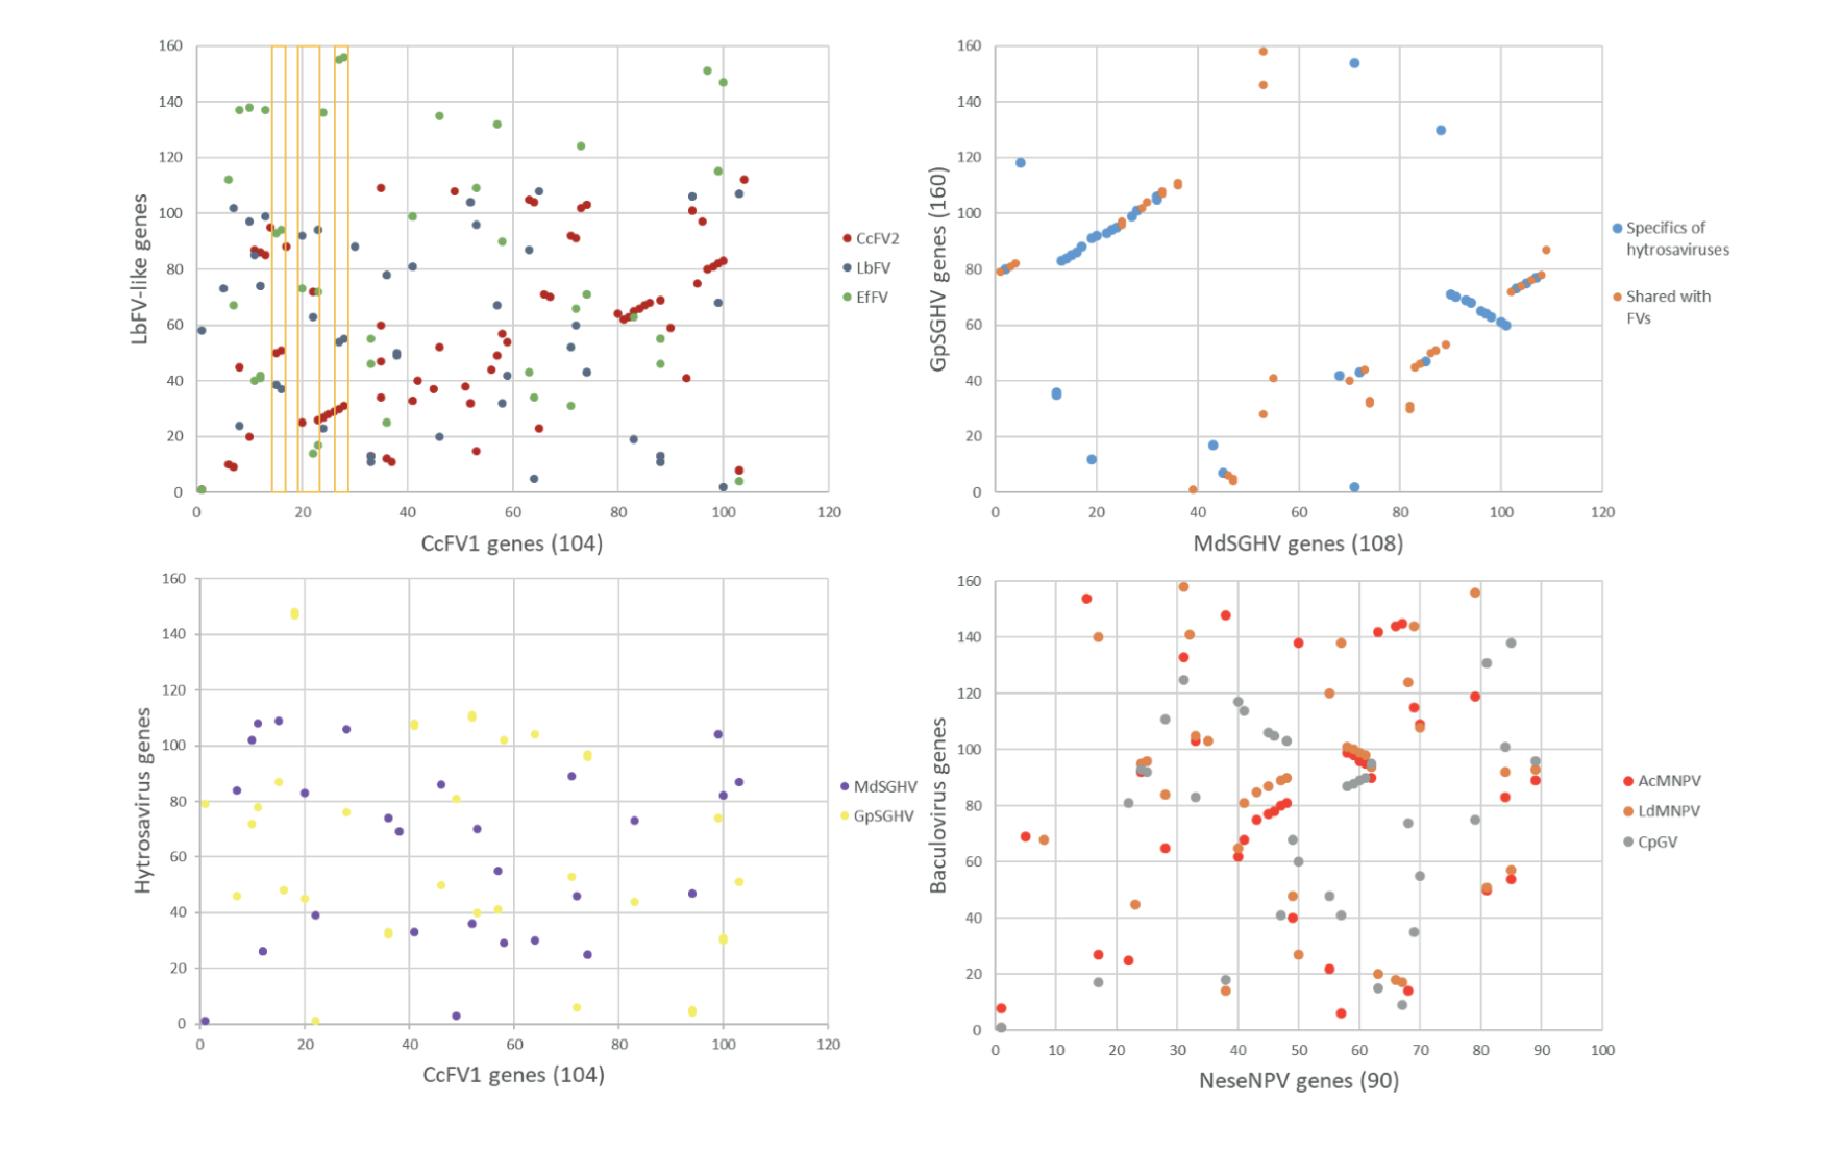
\includegraphics[width=\linewidth,height=\textheight,keepaspectratio]{PhD-master/figures/Syntenic_plot_filamentous.pdf}\centering
\caption[Paper2:Gene order conservation among \textit{Naldaviricetes}]{\textbf{Gene order conservation among \textit{Naldaviricetes} assessed using gene parity plot comparisons}. All genes are represented by dots following the order of the genes in the reference genome on the x-axis, and the positions of the homologs in the other genome on the y-axis. (A) Gene parity plot comparison of the circularized FV genomes. CcFV1 genome is set as reference and its gene order is compared to that of CcFV2 in red, LbFV in deep blue, and EfFV in green. Orange boxes highlight two microsyntenies present in all filamentous viruses presented. (B) GpSGHV-Uga gene organization compared to MdSGHV ones. Genes specific to hytrosaviruses are represented in light blue and genes shared with filamentous viruses in orange. (C) Hytrosavirus gene order relative to CcFV1, with MdSGHV in purple and GpSGHV-Uga in yellow. (D) Gene order comparison between a gammabaculovirus: NeseNPV, two alphabaculoviruses: AcMNPV in red and LdMNPV in orange, and a betabaculovirus: CpGV in grey.}
\label{figure:Syntenic_plot_filamentous}
\end{figure}


\subsection{Filamentous virus distribution in insects}

To gain insights into FV host range, we expanded our search for FV-like sequences to all hymenopterans (n =368 species), dipteran (n = 369 species) and lepidopteran (n = 911 species) by mining genome assemblies available from NCBI and BIPAA (https://bipaa.genouest.org/is/) databases. We also included 32 genome assemblies from endoparasitoid and ectoparasitoid wasps we generated in a previous study (Guinet et al., in review). Diptera and Lepidoptera were chosen because many of them are attacked by parasitoid wasps and may thus be exposed to FVs. We reasoned that mining genomic assemblies may enable us to identify new FVs infecting the specimens used for the sequencing project or endogenous viral elements (EVEs) derived from ancient infections by FVs. To do so, we first queried the 2815 available assemblies (accounting for 1648 species) with the 29 FV-core genes (Github:\href{https://github.com/BenjaminGuinet/PhD_defense/blob/main/Supplementary_paper2/Table%20S4.xlsx}{TabS4}). In a second step, our pipeline aimed at distinguishing free viruses from EVEs by a combination of phylogenetic and contig length metrics (\figurename{\ref{figure:Pipeline_find_filamentous}}). All phylogenies were separately examined in order to verify that the identified sequences were indeed part of the FV clade. In addition, as a given species may be represented by several assemblies, while first pooled together to facilitate initial processing, they were further examined individually when displaying relevant hits. 

The pipeline led to the identification of putative FV core gene sequences in ~10.8\% of the hymenopteran species (n = 40/368 species), ~3,4\% of the lepidopteran species (n = 31/911 species) and ~0.8\% of the dipteran species (n = 3/369 species) (\figurename{\ref{figure:Heatmap_NCBI4}}-B). Correcting for species entry number confirmed that hymenopteran genomes displayed a significantly higher number of putative FV core sequences (twice more than expected) than genomes from the other orders (X2 = 17.4, p-value = 0.00016). Moreover, a striking pattern of positive association between parasitoid lifestyle and presence of FV-like core genes was observed within Hymenoptera: 36 out of 160 parasitoid species were positive for FV-like core genes, whereas only 4 out of 208 free-living Hymenoptera species were positive, which is significantly much more than expected according to a GLS model taking into account the phylogenetic inertia (PGLS : df=1679,  F-value=103.6, pvalue=<.0.0001). All 29 core genes phylogenies can be found in (\href{https://github.com/BenjaminGuinet/PhD_defense/blob/main/Supplementary_paper2/ALL_EVEs_Free-living_filamentous_in_insects.pdf}{ALL\_EVEs\_Free-living\_filamentous\_in\_insects.pdf}).

Depending on the species considered, we were able to detect homologous sequences from one to all the FV core genes. All species with the full (or almost full) set of FV-like core genes corresponded to endoparasitoid Hymenoptera species (\figurename{\ref{figure:Heatmap_NCBI4}}-A). These cases included the parasitoid species \textit{Psyttalia concolor} and \textit{Platygaster orseoliae} for which a previous analysis based on a different pipeline (Guinet et al., 2023, in review) detected the presence of exogenous FV partial genomes (PcFV and PoFV) and FV-like integrated sequences (PoEFV).
\newpage

\afterpage{
\begin{landscape}

 \begin{figure}[]
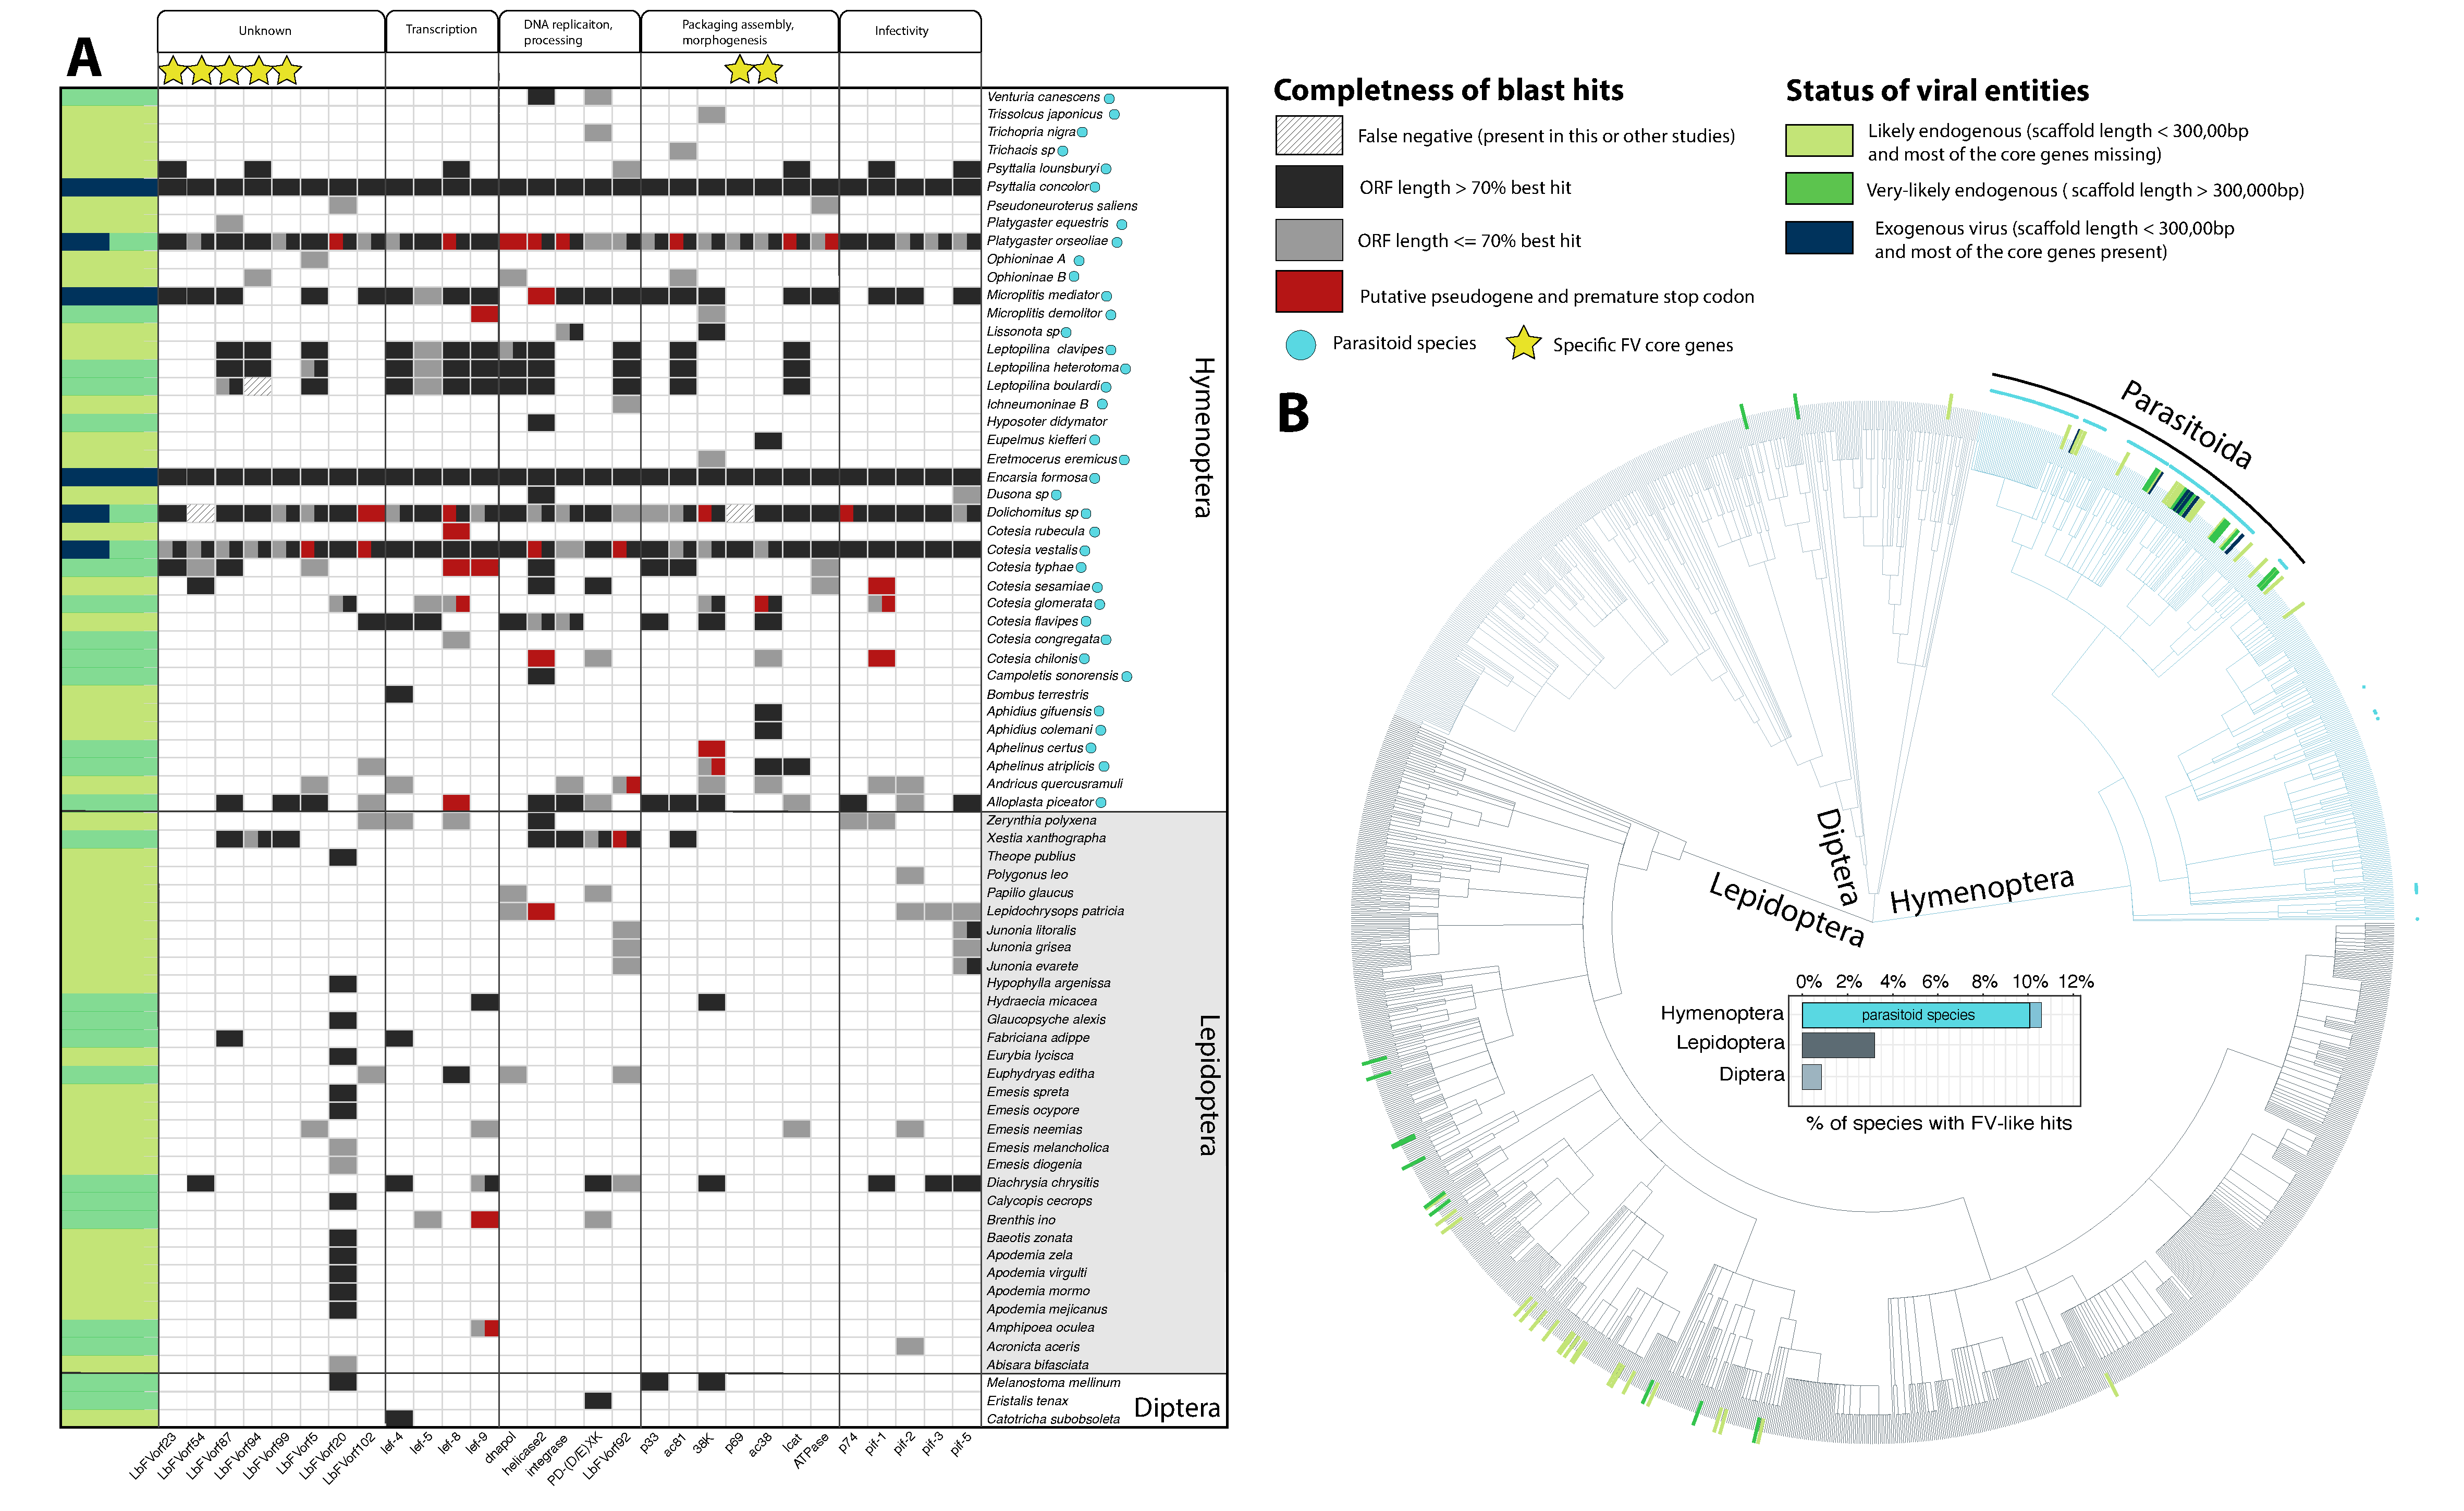
\includegraphics[width=\linewidth,height=\textheight,keepaspectratio]{PhD-master/figures/Heatmap_NCBI4.pdf}\centering
\caption[Paper2:Distribution of endogenous and exogenous filamentous virus among insects]{\tiny\textbf{Set of FV-like sequences identified from different insect orders.} Set of FV-like sequences identified from different insect orders. (A) Table showing presence/absence of putative FV-like core gene homologs in insect genome assemblies from lepidopteran, hymenopteran and dipteran orders using a tBLASTn approach and a phylogenetic validation (note that a given species may be represented by several assemblies derived from different populations). The colors of the boxes represent the ORFs completeness status: black color represents a most probably complete ORF (that spans at least 75\% the size of the best filamentous blast hit), grey color represents a probably incomplete ORF (spanning less than 70\% the size of the best filamentous blast hit), red color represents a pseudogene or an ORF with a premature stop codon, and hatched boxes represent hits further obtained by specific analyses. The presence of two colors in the same box indicates that the genome assembly of the species contains two copies of the same core gene: either complete (black) or not (grey or red). The colors in the left column inform on the probable state of the viral entity: endogenous/exogenous. Several colors in one box indicate the probable presence of both endogenous viral elements and a free-living virus. The cyan circles along the taxon names indicate parasitoid species. (B) The circular phylogenetic tree shows the evolutionary relationships between three insect orders in which branch colors refer to the insect orders: blue = Hymenoptera, light gray = Diptera, dark gray = Lepidoptera. Each colored dash along the leaves of the tree stands for the status of the filamentous elements (green = endogenous FV, dark blue = exogenous free-living FV). The phylogenetic cladogram was reconstructed based of the taxonomical NCBI level of all genomes surveyed in this analysis using the NCBITaxa ete3 function in python. The distribution of the percentage of species having FV-like sequences in each insect order analyzed is displayed within the cladogram inside the phylogeny}
\label{figure:Heatmap_NCBI4}
\end{figure}

\end{landscape}
}

In addition, we found most core genes for three other parasitoid species: \textit{Dolichomitus sp} (Ichneumonidae: Pimplinae) (29/29 tested core genes), \textit{Cotesia vestalis} (29/29) and \textit{Microplitis mediator} (27/29) (Braconidae: Microgastrinae)
(\figurename{\ref{figure:Heatmap_NCBI4}}-A). These results suggest either that FVs have been infecting these parasitic wasps or the presence of well conserved FV-related EVEs in their genomes.To determine the status of these sequences, we used several criteria, in particular (i) the prevalence of the viral sequences in the species (when several individuals of different origin have been sequenced), (ii) the gene density because of the expected difference between viral genomes (high), EVEs (lower) and eukaryote sequences (low), (iii) the cumulative size of scaffolds/contigs carrying the candidate genes compared to the average size of FV genomes, (iv) the presence or absence of pseudogenes and/or cellular genes within the identified scaffolds/contigs. 

On this basis, the data suggest that \textit{Dolichomitus sp} genome contains an endogenous virus and the specimen sequenced were also infected by a FV (\figurename{\ref{figure:Heatmap_NCBI4}}-A, see also \citep{burke_presence_2021}). For \textit{Cotesia vestalis} (diamondback moth parasitoid), we retrieved several assemblies originating from three different sources: Hangzhou (China, \citep{shi_genomes_2019} and Andong (South Korea, \citep{burke_presence_2021}), and Wageningen (Netherland, \citep{gauthier_chromosomal_2021}) and analyzed them further. FV genes were detected in 22 contigs (from 0.9 to 12.1 kb) of the Hangzhou isolate for a total size of 104.3 kb, comprising 78 core and accessory single genes and an average coding density of 87\%. Moreover, as no viral pseudogenes nor cellular genes were found in these contigs, we confirm, as reported by \cite{burke_presence_2021}, that a free-living FV was infecting the Chinese \textit{C. vestalis} isolate, its best relative being CcFV2 (both from similarity of sequences and synteny). In contrast, for the Andong isolate, many of the FV-like core gene sequences (22/29) were found but as a single gene (1/29, \textit{helicase 2}, JZSA01002659) or in clusters with other viral genes on four contigs (from 50 to 97 kb). Some genes were pseudogenized, gene density was relatively low compared to exogenous FV (64-77\% on the two main regions carrying the larger FV gene set) and cellular genes and/or transposable elements could be found nearby (see also \citep{burke_presence_2021}). This isolate therefore likely harbors an endogenous FV integrated relatively recently, but that has already undergone some degeneration. Finally, only a few FV-like core gene sequences could be identified for the Wageningen isolate (7/29) and, except for the \textit{helicase 2}, they were all in the state of remnants. Interestingly, this \textit{helicase 2} gene was not only present alone, within a wasp sequence context, in the two other \textit{C. vestalis} isolates but also in \textit{C. sesamiae}, \textit{C. flavipes} and \textit{C. chilonis} but not in \textit{C. congregata}, \textit{C. glomerata} and \textit{C. rubecula} available genomes, indicating that a much earlier FV integration event occurred  during \textit{Cotesia} speciation.

Further, in the parasitoid \textit{C. flavipes} \citep{gauthier_chromosomal_2021}, nine out of the 29 core genes were detected, the majority of them carried by three scaffolds for a total size of approx 45 kb. Given the high gene density (88.5\%), the absence of pseudogenized viral genes as well as the absence of cellular genes within these three scaffolds, it is plausible that this corresponds to a part of a FV genome, which we found the more closely related to CcFV1. An explanation for the absence of the other core genes would be that the virus genome was not fully covered by the sequencing approach. 

Regarding other hits, it seems likely that they correspond to ancient viral integrations, given that the set of FV-like (core) genes is partial, and/or that the cumulative size of the scaffolds carrying these genes largely exceeds the expected size for exogenous FV genomes (\figurename{\ref{figure:Heatmap_NCBI4}}-A and Github:\href{https://github.com/BenjaminGuinet/PhD_defense/blob/main/Supplementary_paper2/Table%20S1.docx}{TabS1}), and/or that they harbor cellular genes.  \\

Taken together, this data mining pipeline identified a large set of FV sequences in insect assemblies belonging to Hymenoptera, Diptera and Lepidoptera, suggesting that filamentous viruses are  widespread among these insects. However, the prevalence of these FV sequences was higher in Hymenoptera genomes compared to the other orders. Additionally, in the current state of available data, no exogenous FV could be identified in species outside the Hymenoptera order. More strikingly, almost all species positive for FV-core genes have parasitoid lifestyle, and this was true for both presumably exogenous or endogenous sequences. This strongly suggests that FVs are preferentially associated with Hymenoptera parasitoids. Nevertheless, we found FV endogenous sequences in Diptera and Lepidoptera which may have been acquired via parasitism of a hymenopteran host infected with such viruses \citep{muller_genome-wide_2021}. These EVEs are frequently degraded except in two Lepidoptera (\textit{Xestia xantographa} and \textit{Diachrysia chrysitis}) suggesting that most integration events are ancient (\figurename{\ref{figure:Heatmap_NCBI4}}-A). In particular in \textit{D. chrysitis}, FV-like sequences are found as large regions (28 to 106 kb) comprising repetitions of one or two sets of four genes plus unique genes, all flanked by transposable elements. Based on phylogeny analysis, the ancestor behind these integrations would be a FV close to those associated with \textit{Cotesia} genus. However, one gene (LbFV\_orf20) have been frequently retained in a potentially functional state in the Lepidoptera (\figurename{\ref{figure:Heatmap_NCBI4}}-A) suggesting this gene could be used by the corresponding species conferring a new biological function, as described for some bracovirus genes horizontally transferred to Lepidoptera \citep{gasmi_recurrent_2015,di_lelio_evolution_2019}.

\subsection{Unravelling the horizontally acquired genes}

Given that viral genomes are known to hijack genes of various origins by horizontal transfers such as from eukaryotes or bacteria \citep{irwin_systematic_2022, filee_phylogenetic_2008}, we studied the phylogenetic relationships of FV  proteins  sharing similarities with non-viral sequences. Our analyses revealed 23 genes with convincing homologies to proteins from Bacteria, Eukaryotes, and/or Archaea (bit score min = 50 and query coverage min = 25\%). (See phylogeny figures in \href{https://github.com/BenjaminGuinet/PhD_defense/blob/main/Supplementary_paper2/ALL_HGT_filamentous_phyogenies.pdf}{ALL\_HGT\_filamentous\_phyogenies.pdf})

Among them, two were part of the core FV-genes. One of them was the JmjC domain-containing protein (min evalue : 2.8e-14, max evalue : 3.3e-05, G19 Figure S23) and with the other was a putative AAA + ATPase domain (min evalue :2.9e-13, max evalue : 5.9e-05, G43, (\figurename{\ref{figure:JmJC_matthieu}}). Note that JmJC protein had one to two copies per FV genome (LbFV = 2, LhFV = 1, EfFV = 2, PcFV = 1, PoFV = 1, CcFV1 = 2 and CcFV2 = 2).  \\

Concerning JmJC, such proteins are found in organisms from bacteria to human and may be involved in chromatin regulation-related processes (see IPR003347 from InterPro database). Furthermore, it has been reported that a couple of \textit{Mimiviridae} viruses with large genomes encode proteins with the JmJC domain \citep{colson_viruses_2011}. However, no significative homology was found between these viral JmJC-containing proteins and the proteins found in FV-like viruses. Instead, we found only eukaryotic homologs in the databases, which we aligned and used to build a phylogeny (\figurename{\ref{figure:JmJC_matthieu}}). Our phylogenetic analysis suggests that FV homologs would  have been acquired from arthropod genomes (\figurename{\ref{figure:JmJC_matthieu}}). Since the gene tree topology was not inconsistent with a single monophyletic clade containing all FV, (by taking  into account nodes uncertainty) this result suggests that this gene was acquired by the common ancestor of the seven FV genomes (\figurename{\ref{figure:JmJC_matthieu}}, bootstrap support = 71.9). Because of its somehow complicated history due to duplications, and even if at least one homolog is found in each species, we choose not to include it in the list of core genes. Finally, the analysis of domains arrangement clearly showed a virus-specific pattern compared to other homologous sequences, where a final clustering of several zinc finger domains was preceded by the JmJC domain (\figurename{\ref{figure:JmJC_matthieu}}).\\  


 \begin{figure}[H]
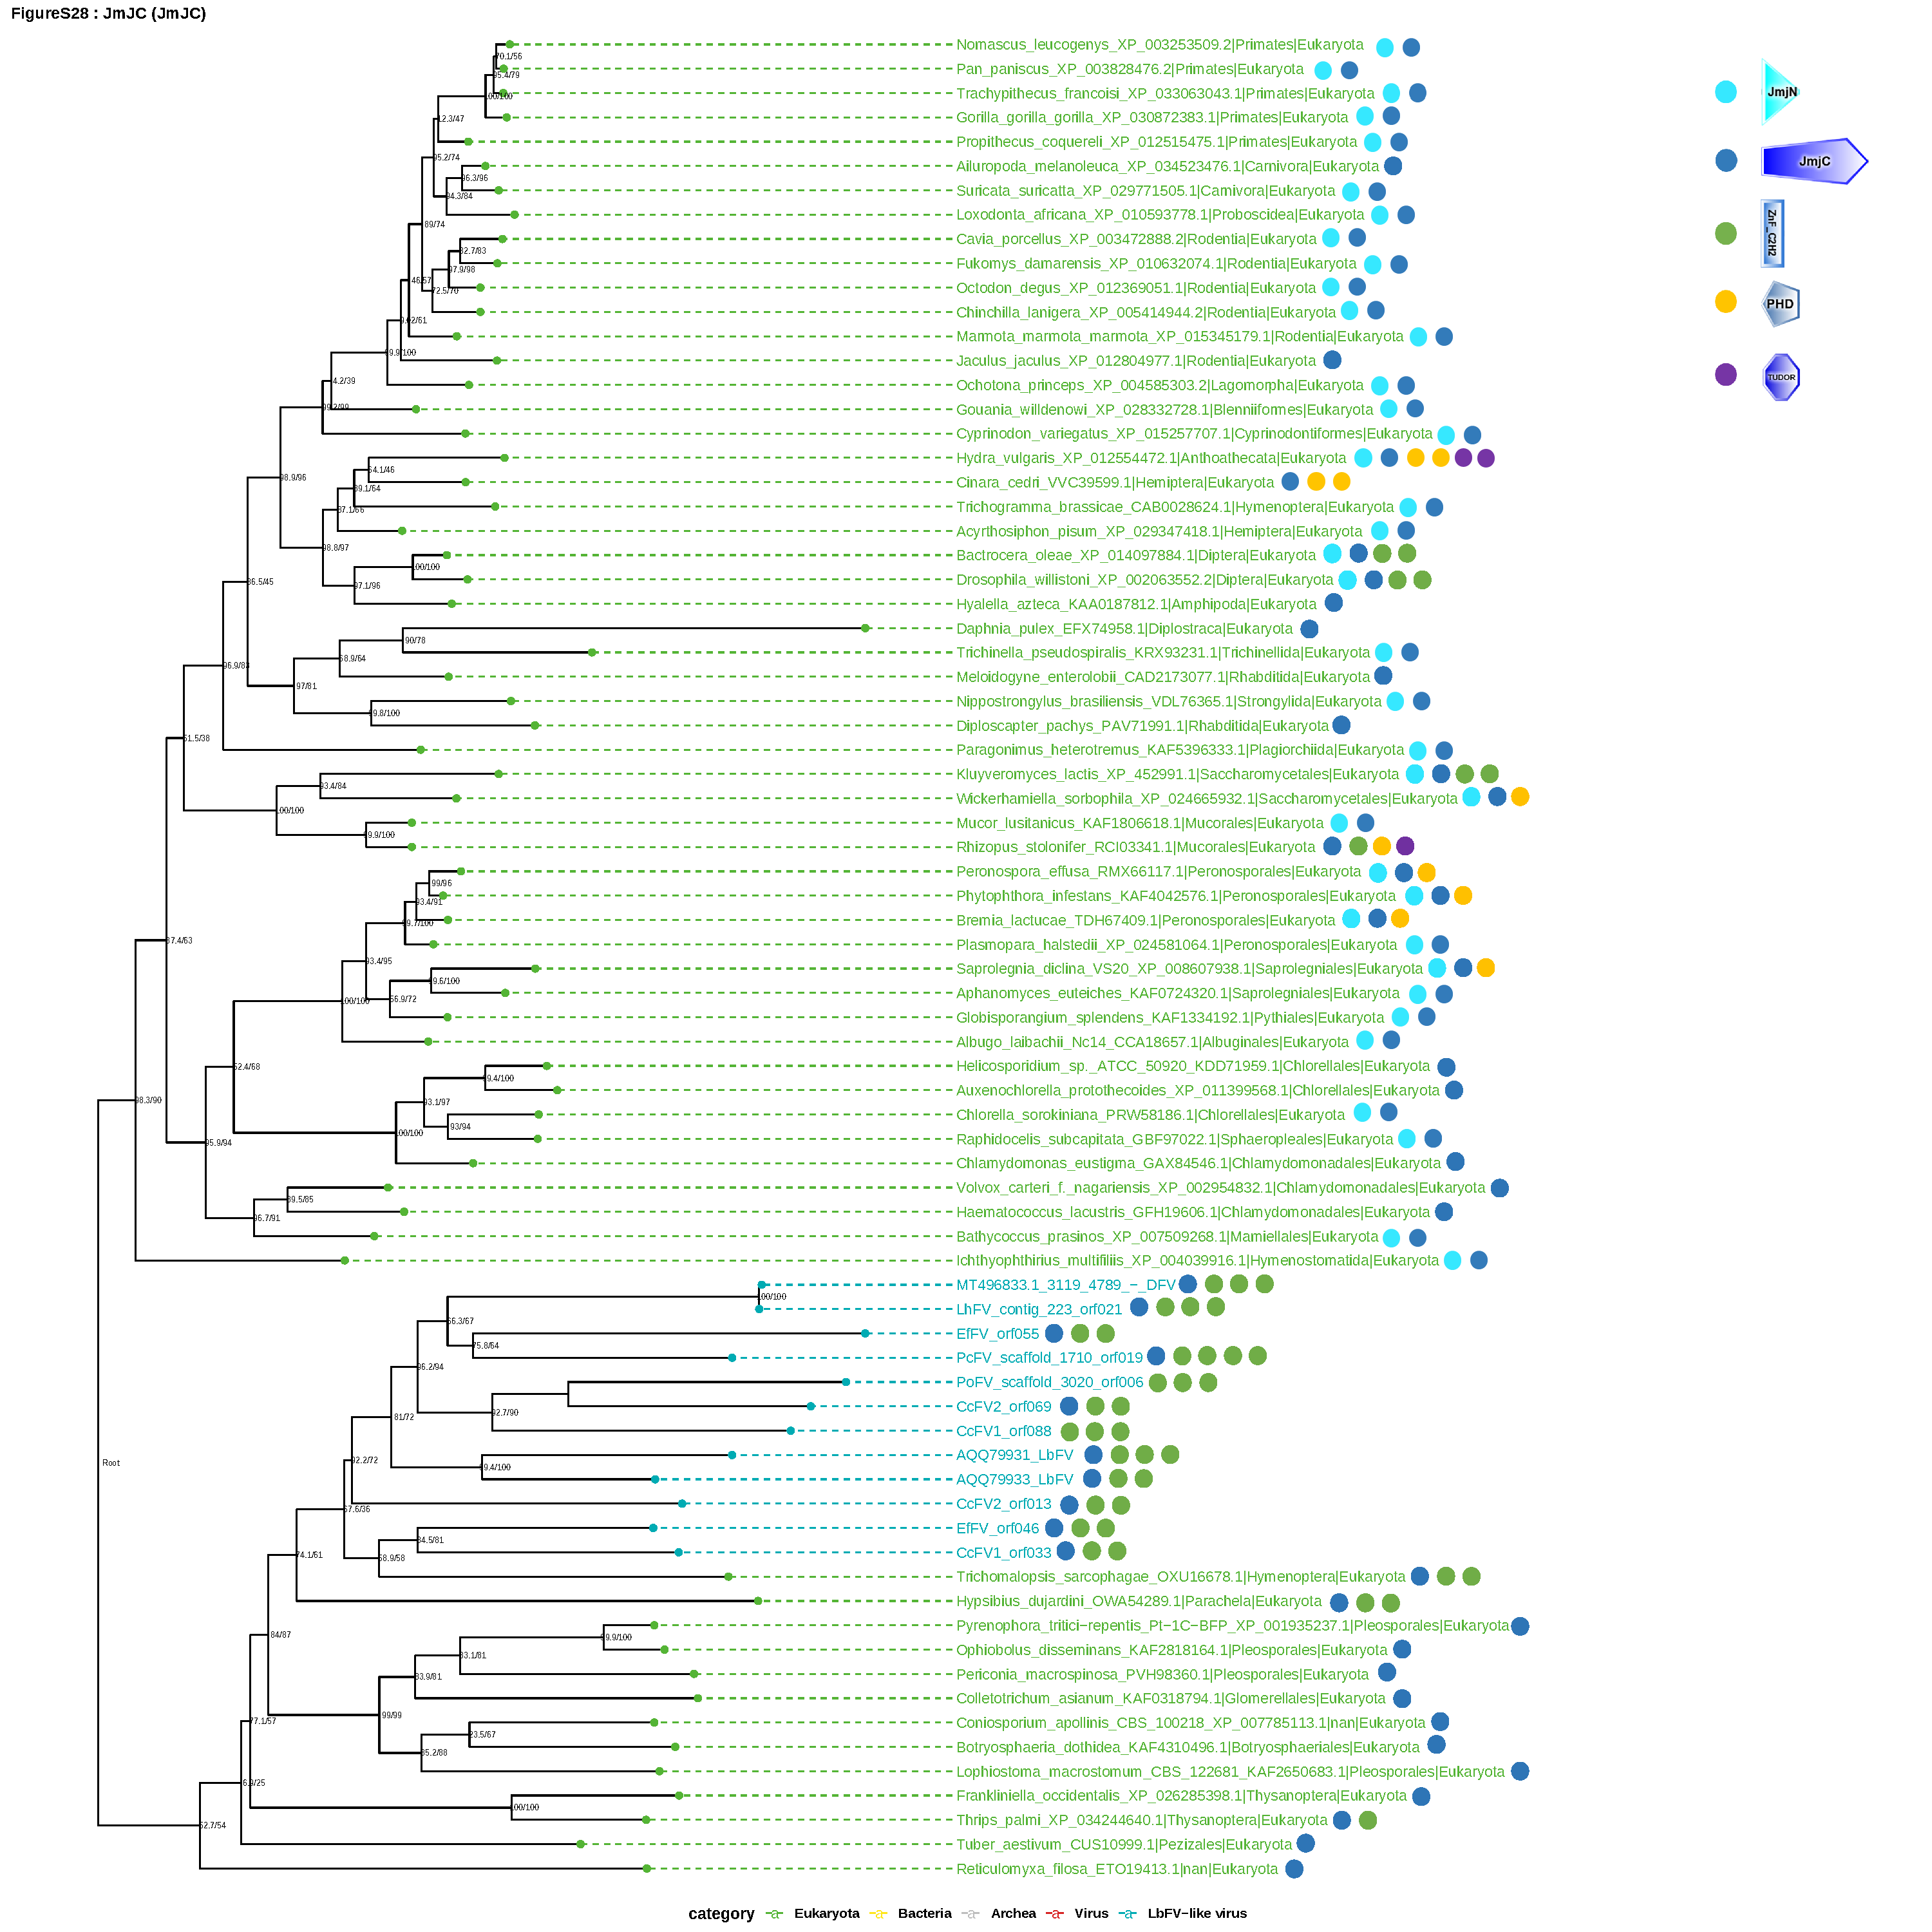
\includegraphics[width=\linewidth,height=\textheight,keepaspectratio]{PhD-master/figures/JmJC_matthieu.pdf}\centering
\caption[Paper2:JmJC filamentous virus phylogeny]{\textbf{JmJC domain phylogeny.} The branches of eukaryotic species are coloured green, while the branches of filamentous viruses are coloured blue. The colorer points adjacent to the species names correspond to a particular domain whose colour code is located in the upper-right corner of the figure.}
\label{figure:JmJC_matthieu}
\end{figure}

ATPase proteins are a large protein family that participate in a variety of cellular processes using the energy from ATP hydrolysis. Given that all filamentous viruses contain this protein, it is possible that it plays a role in supplying the necessary energy for an unknown function. In contrast to JmJC, the AAA+ ATPase genes were present in both FV-like and \textit{Hytrosaviridae} species. The gene phylogeny revealed a well-supported monophyletic clade recapitulating the species phylogeny for these two clades, suggesting that these ATPase genes share a common ancestor at the root of these two families (Phylogeny S10 (GitHub), bootstrap support = 97.3). The identity of the donor is relatively unclear because of the low resolution of the ancient nodes. However, the closest relative of the viral clade \textit{Hytrosaviridae} + FV is a  bacteria, suggesting that this gene may derive from a bacterial gene. On the contrary, we note that the tree topology suggests that the (non-FV) virus AmFV acquired the same gene from an Hymenoptera (Phylogeny S10 (GitHub)).  

Among the 23 putative HGT genes identified, 13 (including JmJC) presented a clear horizontal gene transfer from eukaryotic origin, and one from bacterial origin (G247, Phylogeny S3 (GitHub)). Most of the HGT events, except for JmJC, were unique to one filamentous species. 11 of these genes showed evidence of known functions revealed by a HMMER analysis against the alphafold\_uniprot50 db. Among these genes, we find an inhibitor of apoptosis (G151, Figure S2 (GitHub)), a putative phosphatidate phosphatase (G602, Phylogeny S16 (GitHub)),  a transmembrane protease serine 9-like (G672, Phylogeny S20 (GitHub)), an alpha/beta hydrolase (G486, Phylogeny S22), a dUTP diphosphatase (G704, Phylogeny S15 (GitHub)), a lysozyme (G495, Phylogeny S9 (GitHub)),  a deoxynucleoside kinase (G103, Phylogeny S8), a protein phosphatase (G108, Phylogeny S7 (GitHub)), a beta-1,3-galactosyltransferase (G112, Phylogeny S6 (GitHub)) and a calpain-1 catalytic subunit-like (G149, Phylogeny S5 (GitHub)) (See phylogeny figures in \href{https://github.com/BenjaminGuinet/PhD_defense/blob/main/Supplementary_paper2/ALL_HGT_filamentous_phyogenies.pdf}{ALL\_HGT\_filamentous\_phyogenies.pdf})



\subsection{Filamentous virus morphogenesis}

Abundant long virus particles were observed using transmission electronic microscopy (TEM) throughout the calyx of six \textit{Cotesia congregata} adult females \citep{bredlau_parasitic_2019}, positive in PCR assay for the presence of CcV2 genome. The production of filamentous particles was compared to that of LbFV (\figurename{\ref{figure:Micoscopie_filamentous}}) we reported previously \citep{varaldi_infectious_2003, varaldi_artifical_2006}. The cells that produce CcFV2 are from the same type as those producing bracovirus particles (CcBV). Bracoviruses derive from the endogenization of an ancestral  nudivirus  into the genome of the common ancestor of several subfamilies of braconid wasps. CcFV2-infected cells are homogeneously distributed in the calyx and cohabit with CcBV-producing cells and the calyx lumen is filled with a mixture of filamentous and bracoviral particles (\figurename{\ref{figure:Micoscopie_filamentous}}-J). However, we did not find any cell producing both types of particles at the same time. As described for LbFV  \citep{varaldi_artifical_2006}, replication of CcFV2 occurs in the nucleus where the typical electron dense structure called virogenic stroma are observed, in which virus particles assembly is thought to occur (\figurename{\ref{figure:Micoscopie_filamentous}}-A,B,G). Long electron-dense, non-enveloped rod-shaped nucleocapsids are produced in the nuclei. Their structure is similar to that of LbFV nucleocapsids (\figurename{\ref{figure:Micoscopie_filamentous}}A-D). A slight difference in length can be noted with particles up to 1µm in LbFV \citep{varaldi_artifical_2006} while the longest particle observed in \textit{Cotesia congregata} was 800nm long (not shown), the diameter of LbFV is more than twice that of CcFV2 (45 and 20 nm respectively). The nucleocapsids are released into the cytoplasm by an unknown mechanism (\figurename{\ref{figure:Micoscopie_filamentous}}-C-D). Passage of the nuclear membrane towards the cytoplasm may occur by budding like baculoviruses \citep{granados_vivo_1981}, but this hypothesis is not consistent with the observation of some non-enveloped particles (\figurename{\ref{figure:Micoscopie_filamentous}}-C) and abundant membrane vesicles in the cytoplasm (\figurename{\ref{figure:Micoscopie_filamentous}}-E). Enveloped particles in the cytoplasm and calyx lumen are between 40 and 51 nm in diameter, while LbFV enveloped particles are 60nm in diameter (\figurename{\ref{figure:Micoscopie_filamentous}}). The nucleocapsids of both viruses are often curved (\figurename{\ref{figure:Micoscopie_filamentous}}-C-D) while hytrosaviruses  have  rectilinear virus particles \citep{abd-alla_genome_2008}. The CcFV2 particles in the cytoplasm are usually found in aggregates in which the filamentous particles are aligned parallel to each other (\figurename{\ref{figure:Micoscopie_filamentous}}). This aggregate of particles forms a hexagonal like network with a distance of about 75nm between the particles (center to center) in cross-section (\figurename{\ref{figure:Micoscopie_filamentous}}-E-F). These typical aggregates have already been described in electron microscopy studies of FVs (\figurename{\ref{figure:Table_filamentous_origins}}). Aggregates have also been observed in LbFV infected cells but they involve nucleocapsids in the nucleus (\figurename{\ref{figure:Micoscopie_filamentous}}-B).  Paracrystalline structure of virions are often observed in virus infected cells and might result from physical constraints acting when particles having the same shape are abundant in a compartment. A greater accumulation of LbFV nucleocapsids in the nucleus could result in the formation of aggregates in this subcellular compartment rather than in the cytoplasm. As described in previous studies of Cotesia congragata filamentous virus \citep{de_buron_characterization_1992} and hytrosaviruses (Kariithi PhD dissertation 2013), we observed that nucleocapsids particles were lining the outer membranes of mitochondria near the nuclei in the cytoplasm (\figurename{\ref{figure:Micoscopie_filamentous}}-I). However, the particles do not appear to acquire their envelopes at these sites. Indeed, as in hytrosaviruses, empty membrane vesicles were observed in many cells near the aggregates of CcFV2 particles (\figurename{\ref{figure:Micoscopie_filamentous}}-E), suggesting that the endoplasmic reticulum has a role in the cytoplasmic envelopment of the particles. The extracellular virus has no additional envelope, and no particle aggregate structures were observed in the ovary lumen where filamentous particles are consistently observed in areas containing bracoviral particles (\figurename{\ref{figure:Micoscopie_filamentous}}-J). It is likely that as bracovirus particles, CcFV2 particles are injected into the parasitized host during oviposition (\figurename{\ref{figure:Micoscopie_filamentous}}-J). Indeed, filamentous particles of \textit{Cotesia congregata} have been shown to penetrate a number of host cell types, but no interaction with nuclear pores or replication has been observed  (Stoltz and Vinson 1977). Interestingly it has been shown that the filamentous virus infecting \textit{Cotesia marginiventris}, which is injected by the wasp into the lepidopteran host, is able to replicate in the parasitized host \citep{styer_new_1987}. This raises the question of whether the infection has an effect on the host and the parasitic success of the wasp, as   described for the parasitoid  \textit{Leptopilina boulardi} infected by LbFV \citep{martinez_influence_2012}. 


 \begin{figure}[H]
\includegraphics[width=\linewidth,height=\textheight,keepaspectratio]{PhD-master/figures/Micoscopie_filamentous.pdf}\centering
\caption[Paper2:TEM images of filamentous viral particles]{\textbf{Typical structures observed by electron transmission microscopy (TEM) in cells from two parasitoid wasps infected by filamentous viruses.} (A, C, E) \textit{Cotesia congregata} adult wasp calyx and (B, D, F) \textit{Leptopilina boulardi} adult wasp oviduct (B, D, F). (A, B) Details obtained using higher magnification of the views in the white frames TEM photographs of a calyx cell producing FVs, the white frames represent magnified sections in panels C and E. (C, D) Magnified TEM images of filamentous particles observed within \textit{Cotesia congregata} and \textit{Leptopilina bourlardi} cells, respectively. (E, F) TEM images of typical stuctures showing arrays filamentous particles in Cotesia congregata and \textit{Leptopilina bourlardi}, respectively. N: nucleus and C : cytoplasm. The arrows designate enveloped particles, arrowheads nucleocapsids (in longitudinal section for C, D and cross-section for E, F) and white circle one of the abundant membrane vesicles observed in the cytoplasm. G,H,I J are Electron microscope images showing filamentous particles in \textit{Cotesia congregata} adult wasp. (G) TEM photographs of a calyx cell producing large number of particles, the inset at the bottom right represents a magnified section of the cell nucleus. (H) Images of enveloped filamentous particles obtained using high magnification. (I) Images of a calyx cell producing FVs, the inset at the top left represents a magnified section of the cell cytoplasm. (J) Images of wasp calyx lumen, the inset at the top right represents a magnified section of the lumen containing both filamentous virus and bracovirus particles. TN: nucleus, C:cytoplasm, VS virogenic stroma and N BV: nucleus containing bracovirus particles. White row: enveloped filamentous particle, white arrowheads: mitochondria lined with nucleocapsids, white circle: two bracovirus particles.}
\label{figure:Micoscopie_filamentous}
\end{figure}


\section{Discussion}

In parasitoid wasps, viruses with a particular filamentous shape have been described since the 1970s in multiple species without any idea about their origin. The first fully sequenced dsDNA filamentous virus was the LbFV that infects the endoparasitoid \textit{L. boulardi} \citep{lepetit_genome_2017}. The LbFV genome was found to be phylogenetically close to the \textit{Hytrosaviridae} within the \textit{Naldaviricetes} class, known to infect Dipterans. 

As only one complete genome of a free-living filamentous virus was available, that of LbFV, it was unclear whether the clade deserved the definition of a new viral family, distinct from the \textit{Hytrosaviridae}, as suggested by \cite{lepetit_genome_2017}. Hence, the present study aimed at addressing this question, and additionally at giving further insights into the biology of filamentous viruses. Thus, we have shown that the evolutionary history of this virus clade supports the idea that it belongs to a family closely related to the \textit{Hytrosaviridae} family. In addition, we revealed that these filamentous viruses possess a set of 5 core genes that were exclusive to these viruses, whereas two more core genes (\textit{P6.9} and \textit{Ac38}) were present in some other species families but did not appear to be core genes in these families.  Finally, we gave evidence to support the hypothesis in which filamentous viruses share a singular connection with species of endoparasitoid wasps.\\

\textbf{Biological particularity of FV?}

Among the elements that support the position of the FV-like filamentous viruses within the \textit{Naldaviricetes}, we must first mention that we are dealing with arthropod-infecting viruses that replicate within virogenic stroma found in the nucleus cell. Their large dsDNA genomes are enclosed within large, flexible, rod-shaped enveloped filamentous particles. 

The biology of filamentous viruses, in particular the environment in which the viral particles are produced and their routes of transmission, seems different from \textit{Hytrosaviridae}. Hence, cytological sections demonstrate that \textit{Hytrosaviridae} virus particles replicate in multiple tissues including salivary glands, causing their hypertrophia, which reduces tsetse and housefly reproduction and fertility \citep{abd-alla_tsetse_2011}. Unlike MdSGHV infecting the housefly, where the transmission in strictly horizontal, the replicating GpSGHV virus in the tsetse fly is transmitted both vertically and horizontally by saliva after a blood meal, resulting in a high viral load in the fly colonies \citep{kariithi_hytrosaviruses_2017}. The asymptomatic (or persistent) infection of the tsetse fly GpSGHV may be favourable to GpSGHV by guaranteeing the transfer and maintenance of progeny virus over an extended period of time (fly-to-progeny)\citep{boucias_transgenerational_2013}. 

In contrast, transmission of LbFV from mother to offspring is highly efficient (approximately 95\%) \citep{martinez_competitive_2015}; moreover, the virus effect is limited to manipulating oviposition behavior \citep{varaldi_infectious_2003,varaldi_superparasitism_2005}. Indeed, the LbFV manipulates the oviposition behavior of \textit{Leptopilina boulardi} wasps by inducing superparasitism (laying eggs in already parasitized hosts) \citep{varaldi_infectious_2003}. This behavioral modification promotes horizontal transmission within superparasitized \textit{Diptera} hosts, allowing for the efficient spread of the virus in wasp populations. This way, the virus may reach very high prevalence ($>$90\%) in wasp populations \citep{patot_molecular_2009, patot_prevalence_2010}. In a broader sense, the \textit{Cotesia} species where CcFV1 is found originate from wasp species raised for many years in our laboratory, and there is no evidence of a pathogenic effect, suggesting that filamentous viruses do not have a deleterious effect as strong as in \textit{Hytrosaviridae}.\\
\newpage
\textbf{Unique gene content}

Secondly, a thorough in-depth study of the core gene composition shows that all viruses we have classified in the Filamentoviridae have not only all the prerogatives belonging to the viruses from the \textit{Naldaviricetes} class, but also from the \textit{Lefavirales} order. Indeed, these viruses harbor not only all the requested genes coding for the PIF complex (\textit{p74}, \textit{pif-1}, -2, -3 and -5), as well as a \textit{DNA polymerase} and a \textit{p33} (sulfhydryl oxidase) homologs, but they also harbor homologs coding for the baculovirus late-phase transcriptional complex (three out of the four subunits of the RNA polymerase to which the \textit{lef-5} gene is added), as well as \textit{helicase 2} and \textit{Ac81} homologs which are missing in \textit{Nimaviridae} (ICTV report 2020) (\figurename{\ref{figure:dsDNA_phylogeny_filamentous}}). Our phylogenetic analysis further allowed us to confirm the positioning of these FV-like viruses within the \textit{Lefavirales} order. All Filamentoviridae did form a highly supported monophyletic clade, with \textit{Hytrosaviridae}, as their closest relatives, as expected by previous analysis \citep{lepetit_genome_2017} (\figurename{\ref{figure:dsDNA_filamentous_heatmap}}). Moreover, patristic distances between species in both clades revealed a greater distance between SGHVs and FV-like virus species than within-clade distances (\figurename{\ref{figure:Patristic_distances_filamentous}}).  

Another argument to differentiate this virus clade from other dsDNA viruses belonging to the \textit{Lefavirales} order was the gene content they specifically share. Indeed, all viruses we classified in the Filamentoviridae shared 29 core genes, five of which are FV-like specific (LbFV\_orf23, LbFV\_orf54, LbFV\_orf87, LbFV\_orf94, LbFV\_orf99). Two other FV-core genes (\textit{Ac38} and \textit{P6.9}) were also found in \textit{Hytrosaviridae}, but were not part of the core-genes in this family. Overall, seven core genes (\figurename{\ref{figure:dsDNA_filamentous_heatmap}}, blue columns) were FV - specific, in comparison with the \textit{Hytrosaviridae}, supporting the view that FV represents a different family.   Among these FV-core genes, only the LbFV\_orf37 (\textit{Ac38}) had a known function, in which it is known to negatively regulate viral gene expression in vaccina virus by acting as a decapping enzyme \citep{parrish_characterization_2007}. \textit{Ac38} had also been associated with the budded virus envelope in Helicoverpa armigera nucleopolyhedrovirus \citep{wang_characterization_2005}. All the other genes encode for proteins with unknown function, but surely play an important role in the specific biology of the viruses. \\


\textbf{Parasitoid-filamentous association} 

All Filamentoviridae identified thus far are infecting endoparasitoid wasps. The only exception was DmFV, which was described as associated with a\textit{Drosophila} \citep{wallace_discovery_2021}. However, doubts can be raised on the primary host with which DmFV is actually associated. First, this virus was characterized in only one of the 6668 pool-sequenced Drosophilae explored samples. Second, we highlighted during this study that DmFV and LhFV were 97.98\% identical at the nucleotidic level, 99.999\% at the protein level and had similar GC content (33.5\%).  Additionally, the synteny was almost perfect between DmFV and LhFV (\figurename{\ref{figure:Syntenic_DmFV_LhFV}}). Therefore, it seems quite likely that these two viral entities are in fact the same virus. Since \textit{Drosophila} are attacked by \textit{Leptopilina} species, it is plausible that one of the \textit{Drosophila} sampled by Wallace and collaborator (2021) may have been previously parasitized by an infected \textit{L. heterotoma} wasp; the LhFV would have then been transmitted to the dipteran during oviposition, the developing wasp would then have been eliminated through encapsulation which is frequent in nature \citep{carton_encapsulation_1985}, allowing the parasitized \textit{Drosophila} to reach adulthood. This may explain a misassociation for this virus. If we accept this interpretation, all known FV are infecting Hymenoptera parasitic wasps, and even endo-parasitic wasps (that lay their eggs within their hosts). 

Then, the remaining question is: is this association a simple mirror of our biased investigations (our two research groups are focusing on endo-parasitic wasps), or is this a biological signal? In order to gain insight into this, we systematically looked for FV-like sequences in 2815 publicly available genome assemblies (encompassing 1576 species) among Diptera, Lepidoptera, and Hymenoptera. The 325 Hymenoptera genome assemblies screened included endoparasitoids (n=87), ectoparasitoids (n=29) and many more free-living species (n=209) such as ants or bees. This analysis revealed two striking results. First, signs of infection by a Filamentoviridae, were exclusively found in endoparasitoid species (\figurename{\ref{figure:Heatmap_NCBI4}}-A,B). In addition, signs of endogenization of FV was highly enriched for endoparasitoid genomes (chi2 p-value = 1.381e-14).  Although larger-scale screening for Filamentoviridae viruses using degenerated PCR probes would be required to validate this hypothesis, this result strongly suggests that Filamentoviridae viruses are preferentially infecting endoparasitoid wasps among Hymenoptera. The specific lifestyle of parasitoid hosts may represent an ecological niche favoring virus maintenance and propagation within wasp populations, both vertically from mother to offspring \citep{martinez_additional_2016} and horizontally between unrelated parasitoids sharing the same host \citep{varaldi_infectious_2003}. Aside from demonstrating that these viruses are intrinsically linked to parasitoid species, the presence of numerous endogenous viral filamentous elements (EVEs) in the genomes of many species and specially within endoparasitoid species (\figurename{\ref{figure:Heatmap_NCBI4}}-A,B) indicates Filamentoviridae as a widespread family with many more viral species yet to be discovered. Our pipeline also revealed, albeit to a lesser extent than for Hymenoptera parasitoids, the presence of FV-like EVEs in the genomes of Diptera and Lepidoptera. Since Diptera and Lepidoptera are attacked by Hymenoptera parasitoids, this may reflect recurrent viral gene transfer from infected parasitoids to their hosts. Although this idea may have been considered as unrealistic a few years ago, our conception has changed, since various studies revealed the occurrence of horizontal gene transfer between parasitic wasps and their (Lepidoptera) hosts mediated by endogenized viruses \citep{gasmi_recurrent_2015,di_lelio_evolution_2019,muller_investigating_2022}. The question of whether these viruses also replicate in other species, such as Lepidoptera or Diptera, remains to be investigated. Prior study uncovered evidence of Lepidoptera-replicating filamentous viruses \citep{styer_new_1987}, but since no sequencing was available for these viruses, we cannot be certain that they belong to the Filamentoviridae family. Therefore, we prefer not to draw the conclusion that filamentous are specific to endoparasitoids Hymenoptera, and instead propose that filamentoviruses are preferentially found in endoparasitoid Hymenoptera species. Interestingly, among the EVEs found in Diptera and Lepidoptera, some appear to be intact and thus potentially functional in the hosts. A functional analysis of these sequences may shed light on their potential function for the organism. 


\section{Conclusion} 

All together, these results support the Filamentoviridae as a new family distinct from the \textit{Hytrosaviridae} and allows us to propose the Filamentoviridae as the 4th viral family in the \textit{Lefavirales} order, along with the \textit{Hytrosaviridae}, the \textit{Nudiviridae} and the \textit{Baculoviridae} families. Further research will be needed to fully explore the association between these viruses and their parasitoid hosts and gain a better understanding of the role of filamentous viruses in parasitoid-virus interactions. 

Since FV appear to be closely associated with endoparasitoid wasps, one remaining question is whether and how these viruses affect the biology of parasitoids, and conversely how these viruses adapted to this peculiar parasitoid lifestyle. As evoked previously, the only FV for which we have detailed information on its biology is LbFV. This virus manipulates the superparasitism behaviour of the wasps, thus spreading in populations.  One open question is whether this behavioral manipulation could be a trait shared by some or all Filamentoviridae members, as all hosts provide the same opportunity for viruses to be transferred horizontally. A previous study looked for LbFV genes involved in \textit{L. boulardi} oviposition behavior manipulation \citep{varaldi_deciphering_2018}. In this transcriptomic study, \textit{L. boulardi}'s abdomen and head expressed 20 ORFs differently in presence of the virus \citep{varaldi_deciphering_2018}. Two of these 20 behavior manipulation candidate genes were found in the Filamentoviridae unique core gene set (LbFV\_orf94 and LbFV\_orf37 (\textit{Ac38})). Although these genes are only candidates involved in the behaviour manipulation, this opens the possibility that they may be involved in behavior manipulation in all Filamentoviridae. Clearly, other phenotypic data and functional tests involving other FV-infected wasps are needed to further test this idea.

\section{Material and methods}

\subsection{Sampling} 

The six filamentous viruses characterized in this study are associated with five endoparasitoid wasp species belonging to four distinct Hymenoptera families: \textit{Cotesia congregata} (Hymenoptera, Braconidae), \textit{Encarsia formosa} (Hymenoptera, Aphelinidae), \textit{Psyttalia concolor} (Hymenoptera, Braconidae), \textit{Platygaster orseoliae} (Hymenoptera, Platygastridae) and \textit{Leptopilina heterotoma} (Hymenoptera, Figitidae). They were named as follows: Cotesia congregata filamentous virus 1 (CcFV1), Cotesia congregata filamentous virus 2 (CcFV2), Encarsia formosa filamentous virus (EfFV), Psyttalia concolor filamentous virus (PcFV), Platygaster orseoliae filamentous virus (PoFV), and Leptopilina heterotoma filamentous virus (LhFV). Among these viruses, only the LhFV partial genome was sequenced after virus purification done for a former metagenomic work (Varaldi et al., \textit{in prep}). The others were obtained alongside wasp sequencing projects (\figurename{\ref{figure:Table_genomes_filamentous}}). 

Cotesia congregata filamentous viruses were identified from two \textit{Cotesia congregata} distinct populations \citep{bredlau_parasitic_2019}, CcFV1 being associated with our well-established laboratory strain (MsT wasp) reared on its natural host, \textit{Manduca sexta} (Lepidoptera, Sphingidae), fed on a synthetic tobacco-based medium; and CcFV2 being associated with another \textit{C. congregata} species (CcC wasp), specialized on \textit{Ceratomia catalpae} (Lepidoptera, Sphingidae) feeding on mature \textit{Catalpa} trees (\textit{Catalpa speciosa} Warder). MsT wasp DNA was extracted as previously described \citep{gauthier_chromosomal_2021} from a restricted number of haploid males issued from a single virgin female to reduce genetic diversity. CcC wasp DNA was extracted from a single brood using the Geneclean Turbo 96 kit (Q-BIOgene) according to the manufacturer’s instructions. Several approaches were then used to sequence both wasp genomes: a 454/Illumina combined sequencing approach at the Genoscope platform (Evry, France) for MsT \citep{gauthier_chromosomal_2021} and a PacBio Sequel sequencing approach at University of Delaware sequencing lab (USA) for CcC  (\figurename{\ref{figure:Table_genomes_filamentous}}). 

\textit{P. concolor} DNA was extracted from single female, while \textit{E. formosa} and \textit{P. orseoliae} were a mix of dozens of individual females in order to obtain enough DNA using the NucleoSpin Tissue extraction kit (Macherey-Nagel). The DNAs were used to construct Illumina TruSeq Nano DNA library sequenced as paired-end (2x150bp) at the GenoToul platform (Toulouse, France). Leptopilina heterotoma filamentous virus in contrast, was extracted following a purification protocol relying on filtration coupled with enzymatic treatments as described in \citep{lepetit_genome_2017}. The DNA was extracted using the same kit and sequenced on an Illumina platform at Macrogen (paired-end 2x 150bp).  

In addition, long read sequencing was performed on \textit{E. formosa} to obtain the complete EfFV genome. DNA extraction was performed on 100 individuals using the Blood and Cell Culture DNA minikit kit, Qiagen. Sequencing was done using the MinION spk-lsk109 protocol. A wash buffer was used after ligation of LFB adapters. Final elution was done on 30µl with a final concentration of 90.4 ng/µl (qubit). We then used 15µl of DNA for deposition on the flow cell. 


\subsection{Electron microscopy analyses}

For \textit{Leptopilina}, ovaries of females were fixed for 2 hours in a solution of 2\% gluteraldehyde buffered with 0.1 M sodium cacodylate (pH 7.4) and post-fixed in 2\% osmium tetroxide in the same buffer for 1 hour (room temperature). Tissues were then dehydrated in a series of graded acetones and embedded in Epon’s medium. Sections were cut on a LKB ultratome. Thin sections were double stained in uracyl acetate and lead citrate. They were examined with a Zeiss EM 10CR transmission microscope at 80kV. 

For \textit{Cotesia}, samples were fixed in mixture of 2\% paraformaldehyde, 2\% glutaraldehyde and 0.1\% sucrose in 0.1 M cacodylate buffer (pH 7.4) for 24 h, washed 3 times for 30 min in 0.1 M cacodylate buffer, and postfixed for 90 min with 2\% osmium tetroxide in the same buffer. After washing in 0.1 M cacodylate buffer for 20 min and 2 times for 20 min in distillated H2O, samples were dehydrated in a graded series of ethanol solutions (50\% ethanol 2 times for 15 min; 70\% ethanol 2 times for 15 min and a third portion of 70\% ethanol for 14 h; 90\% ethanol 2 times for 20 min; and 100\% ethanol 3 times for 20 min). Final dehydration was performed by 100\% propylene oxide (PrOx) (VWR Int) 3 times for 20 min. Then, samples were incubated in PrOx/Epon epoxy resin (Fluka) mixture in a 2:1 ratio for 2 h with closed caps, in PrOx/Epon epoxy resin mixture in a 1:2 ratio for 2 h with closed caps and 90 min with open caps, and in 100\% Epon for 16 h at room temperature. Samples were replaced in new 100\% Epon and incubated at 37°C for 24 h and at 60°C for 48 h for polymerization. Ultrathin sections (thickness, 70 nm) were cut with a Leica Ultracut UCT ultramicrotome (Leica Microsystems GmbH), placed on transmission electron microscope (TEM) one-slot grids (Agar Scientific) coated with Formvar film, and stained 20 min with 5\% uranyl acetate (Electron Microscopy Science) and 5 min with Reynolds lead citrate. The sections were then observed at 100 kV with a JEM-1011 TEM (JEOL) connected to a CMOS Rio 9 digital camera driven by Digital Micrograph software (Gatan). 

\subsection{Genome sequencing and assembly}  

The paired-end reads were quality trimmed using fastq-mcf tool with the following parameters: -q15 --qual-mean 30 -D150 (https://github.com/ExpressionAnalysis/ea-utils) and assembled using IDBA-UD \citep{peng_idba-ud_2012}. Typical scaffolds coming from filamentous-like free-living viruses were then defined on the basis of (i) at least one homology to a LbFV ORF and (ii) a significant coverage deviation (corrected empirical p-value) compared to the coverage depth distribution of BUSCO genes (analysis performed with BUSCO v3 based on BUSCO genes shared by all arthropods) \citep{manni_busco_2021}. We were thus able to characterize 14, 9, and 6 putative viral scaffolds from \textit{P. orseoliae} (i.e., PoFV), \textit{P. concolor} (i.e., PcFV) and \textit{E. formosa} (i.e., EfFV) sequencing data, respectively.  

The EfFV viral genome was further circularized using both MinION long reads (Oxford Nanopore Technologies) and the previously obtained Illumina short reads. Nanopore adapter were removed using Porechop v0.2.4 \citep{wick_completing_2017}, read quality was controlled using NanoPlot v1.33.0 \citep{de_coster_nanopack_2018} and poor-quality reads trimming was done using NanoFilt v2.6.0 \citep{de_coster_nanopack_2018} (-q 12 --headcrop 75). The assembly was first performed with Flye v2.9-b1774 algorithm \citep{kolmogorov_metaflye_2020} (-meta -scaffolds) then polished with racon v1.4.3 \citep{vaser_fast_2017} (2 rounds of polishing using Minimap2 v2.24 for mapping \citep{li_minimap2_2018}) using raw reads from Illumina TruSeq Nano DNA library. This allowed to reduce the number of scaffolds from six to two. Next, we isolated all R1 and R2 Illumina reads as well as the trimmed Nanopore reads that had a convincing homology with one of these two contigs (mmseqs2 search --search-type=3, Evalue max = 9e-13, db = reads, query = the two contigs) then submitted them to the Unicycler pipeline \citep{wick_unicycler_2017} which generated a single contig assembly graph showing circular string graphs, thus revealing the circular DNA structure of the full-length EfFV genome. 

The genome of Cotesia congregata filamentous virus 1 (CcFV1) was isolated following sequencing of a laboratory strain of \textit{Cotesia congregata} (reads available on ERS4256209). Illumina paired-end and 454 (single-end and 3-8-20kb Mate-pairs) reads (available on ERS4256209) were filtered for quality and trimmed using CutAdapt v.3.5 \citep{martin_cutadapt_2011} (-q 20,20 –e 0.10 --max-n 0.5 --minimum-length 30). Additionally, 454 reads were trimmed for homopolymers with a minimum length of eight nucleotides using NGS QC Toolkit v2.3 \citep{patel_ngs_2012}. The genome of Cotesia congregata filamentous virus 2 (CcFV2) was retrieved following PacBio Sequel sequencing of \textit{Cotesia congregata catalpae} strain. 

\textit{De novo} reconstruction of complete FV genomes in \textit{C. congregata} subspecies was done by identifying reads of interest through homology search against  LbFV ORFs (seed). Alignments of processed reads on host genomes and “seeds” were performed using BLASR v5.3.5 \citep{chaisson_mapping_2012} for PacBio reads and bowtie v2 2.3.5.1 (with “local” parameters) \citep{langmead_ultrafast_2009} for Illumina and 454 reads. Mapped reads on respective "seeds" were then \textit{de novo} assembled using Trycycler v0.5.1 \citep{wick_trycycler_2021} and Unicycler v0.4.8 \citep{wick_unicycler_2017} to reconstruct respectively CccFV and Cc-labFV genomes. Assembled reads were then realigned to evaluate quality and circularity of obtained FV assemblies. Alignment results were visualized using Qualimap v2.2.2 \citep{okonechnikov_qualimap_2015} and IGV \citep{robinson_integrative_2011}. Finally, host genomes and generated FV assemblies were visualized with Blobtools v1.1.1 \citep{laetsch_blobtools_2017} using taxon-annotated GC-coverage plots. The assembler produced assembly graphs showing circular string graphs, thus revealing a signature of FV circular DNA structure. \textit{De novo} assembly of CcFV1 454 mate pairs (3, 8 and 20kb) were aligned following forward-forward orientation with the expected insert sizes according to the 454-mate pair sequencing protocol. About 94\%, 80\% and 72\% of respectively 3Kb, 8Kb and 20Kb reads were aligned in a proper way, while respectively approx 6\%, 20\% and 28\% were aligned discordantly (opposite orientation). Discordant reads line up around the two ends of the scaffold\_281 with much larger insert sizes until approx 90Kb, revealing thus a circularization signature at both ends of the scaffold sequence. Aligned reads on scaffold\_281 (Illumina and 454 single end reads) were then \textit{de novo} assembled using Unicycler v0.4.8 \citep{wick_unicycler_2017}. The assembler generated a fragmented genome assembly composed of 4 contigs with a total length of 100,616 nt and a N50 length of 29,109 nt. The assembler was thus unable to reconstruct the full genome of Cc-lab-lineFV. Nevertheless, obtained contigs aligned perfectly on the scaffold\_281 (101,121 nt) and one of the 4 contigs spanned the two ends of the scaffold with a hit length of 23,379 nt. Assembly graphs, even if they were fragmented, showed circular string graphs revealing a circular signature of FV cDNA structure. 

\subsection{Gene prediction and annotation} 

Several tools were combined to obtain the most standardized and accurate gene prediction across all our fully and partially sequenced FV genomes. In a first step, a \textit{de novo} prediction of all potential ORFs was performed under Geneious Prime (2019.2.3) \citep{kearse_geneious_2012} starting from the first detected ATG codon to the STOP codon. Only ORFs with a length greater than or equal to 150 bp were kept. The inner ORFs were not considered. In a second step, complementary ORF predictions were performed using both VGAS v1 (params : -i=1 -n -p -l 150) \citep{zhang_vgas_2019} and Prodigal v2.6.3 (default parameters) \citep{hyatt_prodigal_2010}. Finally, were only kept ORFs confirmed by both the Geneious prediction tool and at least one of the two other predictive methods (generally both Prodigal and VGAS confirmed Geneious proposal). Taking these parameters into account, for LbFV genome, we lose nine ORFs among those initially predicted and published (LbFV\_orf12, orf16, orf34, orf40, orf45, orf46, orf57, orf64 and orf95). 

In a few cases, considering alternative START codons like TTG or CTG, it was possible to define for a given species either new (\textit{lef-5} gene) or longer ORFs (e.g. \textit{lef-9} and \textit{lef-4} genes, whose sequence is more consistent with those predicted in other viral species). Such use of alternative codons has been validated in Hytrosaviruses \citep{abd-alla_comprehensive_2016} and is suggested for some FV genes by the prodigal predictions. However, since these predictions cannot be supported by transcriptomic data (not available to date), they were not retained for our overall analysis (only taken at the margin in the core gene set and the synteny analyses). Additionally, by in depth manual inspection, we identified ORFs corresponding to \textit{P6.9} homologs. Indeed, such genes are difficult to detect by classical tools as they are most of the time located in low complexity regions and thus hidden in bioinformatic pipelines, moreover they can have a size of less than 150 bp. 

ORF similarities were identified using BLASTP, BLASTX and/or TBLASTN \citep{altschul_gapped_1997,altschul_protein_2005}  against either the whole NCBI non-redundant protein database, the NCBI non-redundant protein database restricted to virus taxons (taxid:10239) or against a local database composed of either all the predicted ORFs or all the genomic sequences using the BLAST tool from Geneious Prime (2019.2.3). Further similarites and ORF assignement were infered based on detected functional domains identified by domain search using either the Interproscan (https://www.ebi.ac.uk/interpro/, Blum et al., 2020) tool plugin from Geneious or probabilistic methods like HHpred or HMMER from the MPI Bioinformatics Toolkit of the Max Planck Institute (https://toolkit.tuebingen.mpg.de).  

\subsection{Clusters of homologous sequences} 

Based on the homologies between ORFs, clusters of homologous sequences were established (clustering every ORF with at least a bitscore $>$ 40) following a all-vs-all blastp search on mmseqs2 \citep{steinegger_mmseqs2_2017} (more details in \figurename{\ref{figure:Pipeline_filamentous_phylogeny}}). Following this, we carried out a second, more sensitive clustering process. As a result, we created profiles for each of the clusters (HMMER profile v3.3.2). Then, HMMER search was used to do a HMMER search between all cluster profiles and the initial database (all ORFs). We integrated the cluster from which the ORF originated with the cluster from which the profile derived if one or more ORFs had convincing hits (e-value max = 9e-05) with one or more clusters. In this step, homologous ORFs that were not grouped in the same cluster because of the stringency were combined. The e-value parameters were optimized to obtain complete expected clusters with the 29 core gene set present in (Github:\href{https://github.com/BenjaminGuinet/PhD_defense/blob/main/Supplementary_paper2/Table%20S4.xlsx}{TabS4}). We counted the number of loci present in more than two copies among the clusters to guarantee that the second clustering process did not build multiple non-paralogous proteins sharing homologous domains. Clusters with more than four duplicated copies and more than 70\% of the loci duplicated were reanalyzed using more stringent clustering (bit score min = 100). (e.g. \textit{pif-3} and \textit{pif-1} were assigned to the same cluster in the second step and were split into two separate clusters using this rule). Among the clusters chose during the phylogenetic inferences, we only selected one paralogue/species when multiple paralogues were found (choosing the one with the best evalue compared to the LbFV homolog). Finally, all potential homologs (both within-filamentous viruses but also with related viruses) were confirmed by a thorough examination of their sequence alignment. When a homolog could be missing in a species a reverse blast search from a consensus sequence was performed. Some potential homologs for which the alignment was less obvious could also be conserved on the basis of the synteny observed with the neighboring ORFs (see paragraph below). Finally, ORFs were named according to the similarities encountered either with genes of known function, or with conserved protein domains, or with genes of unknown function already identified in LbFV. For all other ORFs they were named according to their position within the genome of the virus to which they are attached for the full-length genomes (virus species name\_position) or within the contig or scaffold on which they were found for the partial genomes (virus species name\_scaffold/contig number\_position). 

\begin{figure}[!htpbt]
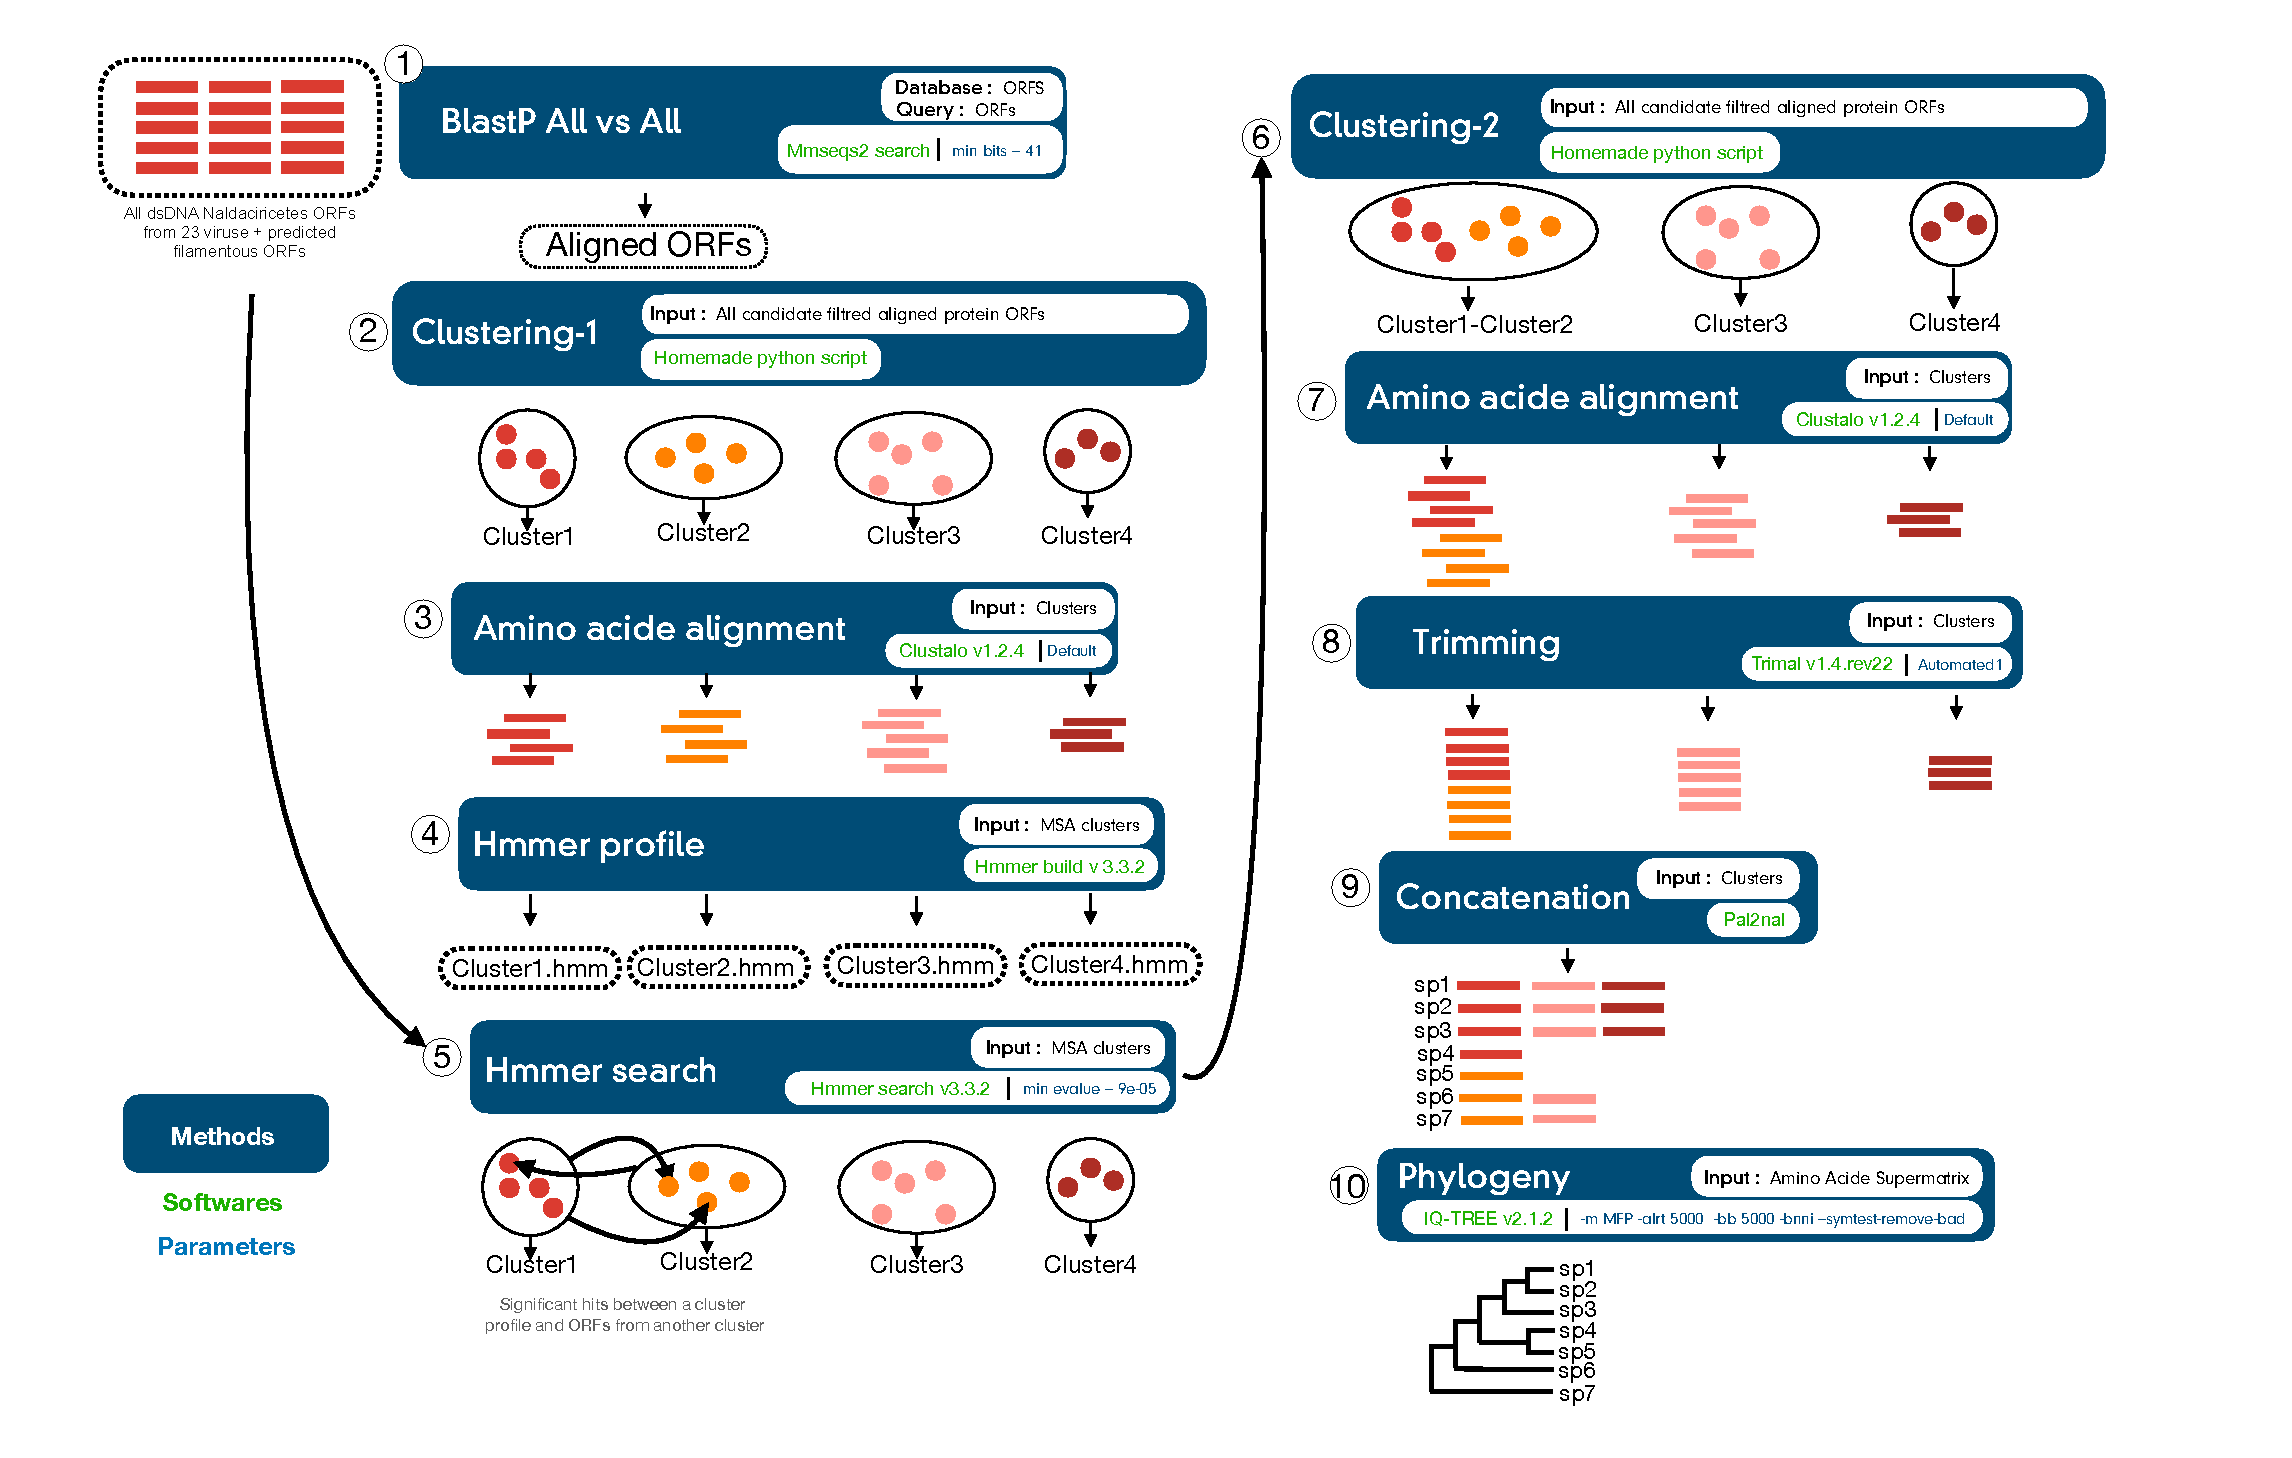
\includegraphics[width=\linewidth,height=\textheight,keepaspectratio]{PhD-master/figures/Pipeline_filamentous_phylogeny.pdf}\centering
\caption[Paper2:"All-gene" method pipeline abstract]{\textbf{Graphical description of the steps taken to obtain the "all-gene" phylogeny}. First, an all-vs-all BlastP using mmseqs2 search \citep{steinegger_mmseqs2_2017} was conducted between all predicted \textit{Naldaviricetes} ORFs in our study (1). Then, a first clustering step was carried out based on a shared alignment with a score of at least 40 bits and a 25\% alignment coverage (2). The resulting clusters were then aligned using ClustalO (v1.2.4) \citep{sievers_clustal_2018} (3). Since it was possible that two homologous clusters were not brought together during the initial clustering stage, a second clustering step employing more sensitive HMMer profiles was then performed to bring the clusters together (4). If at least one protein in a cluster had a Hmmer alignment with an evalue less than 9e-5, the two clusters were merged into one (6). At this time, it was possible that we have incorrectly put together clusterd because of conserved domains between non-homologous proteins. To counteract this, we hypothesised that a viral species should contain few paralogs of the same gene within a cluster. Therefore, if a cluster contained more than three paralogs in more than 70\% of the cluster's species, we repeated step 5 with a increasingly bitscore value until we got a cluster with a number of paralogs per species below this criterion. Then, we aligned the clusters in the protein space using ClustalO (v1.2.4) \citep{sievers_clustal_2018} (7) and trimmed the cluster alignments using Trimal (v1.4rev22) \citep{capella-gutierrez_trimal_2009} (8). Using the pal2nal tool \citep{suyama_pal2nal_2006}, we concatenated the collection of alignments (partitions) comprising more than four species into a single supermatrix. Finally, using the tool Iqtree2 (v2.1.2) \citep{minh_iq-tree_2020}, we inferred the phylogenetic tree of the partitions of genes by using for the best evolutionary model for each partition.}
\label{figure:Pipeline_filamentous_phylogeny}
\end{figure}


In the "all-genes" phylogenetic analysis, only clusters with at least four viral species were kept. In the "core-genes" method 29 core genes defined in (\figurename{\ref{figure:dsDNA_phylogeny_filamentous}}) (i.e., ORFs present in the seven FV-like viruses (minus DmFV)) were used. 

\subsection{Synteny analyses}

The comparison of gene order was performed on the basis of the homologous relationships reported in the annotations of the different published virus genomes as well as the virus genomes described in this study.  Duplicated genes were assigned to a single gene in the reference genome used for the plot. Genes were compiled in a correspondence table using Microsoft Office Excel in order to compare positions between viruses. Then gene parity plots drawn from this table also took into account the homologs and specific genes between the different families by highlighting them in different colors. For viruses whose genomes were not circularized, the different clusters were linked for analysis by comparing the order of their numbering; the different clusters can be visualized on the gene parity graph by following the corresponding color code. 

From the gene plots, we designed a score to evaluate the level of conservation/fragmentation of the gene order. The Synteny score indicates the level of order conservation (Sc) and reciprocally the Fragmented score (Fc) indicated the fragmentation level. The calculated score takes into account the number of homologous genes (Hn), the number of genes in synteny (NgS) and the average number of genes in syntenic blocks (AgSB). The syntenic blocks were defined from the tables of gene plots by allowing a jump and/or an inversion of two genes for the different series.     

\subsection{Insect dsDNA virus phylogenetic analysis}

In order to infer the phylogeny of \textit{Naldaviricetes} dsDNA viruses, two distinct datasets were processed. First, a custom clustering pipeline was created using an "all-genes" method (see (\figurename{\ref{figure:Pipeline_filamentous_phylogeny}}) for an abstract details). This pipeline included a BlastP search between all accessible and predicted ORFs in the 25 dsDNA viruses used for this investigation (min bit = 41, min evalue = 2.5e-06) (7 \textit{Nudiviridae}, 5 \textit{Baculoviridae}, 3 \textit{Hytrosaviridae}, 8 LbFV-likeFV-like, 1 AmFV-like and 1 WSSV used as outgroup) (see supplementary excel file: “\textit{Naldaviricetes}” spreadsheet). The third used \textit{Hytrosaviridae} was the partially sequenced Drosophila-associated salivary gland hypertrophy virus (DmSGHV) for which we improved step-by-step core gene and also nearby gene sequence assemblies using a tblastN strategy with the MdSGHV proteins as a bait, the 14 available sequence fragments from the Drosophila-associated salivary gland hypertrophy virus (MT469997 to MT470014, \citep{wallace_discovery_2021} and the corresponding Drosophila melanogaster SRA library (SRX5299040). 

In both “all-genes” and “core-genes” approaches, the ORF clusters were aligned with Clustal-Omega v1.2.4 \citep{sievers_fast_2011} in the protein space and trimmed with Trimal v1.4.rev22 (options: automated1) \citep{capella-gutierrez_trimal_2009}. Each ORF cluster was concatenated to generate a super-matrix with various partitions. A maximal symmetry test \citep{naser-khdour_prevalence_2019} was used to eliminate heterogeneous partitions (p-value cutoff 0.05). We inferred the phylogenetic tree in both approaches using a Maximum-likelihood framework (ML) implemented in IQ-TREE 2.1.2. \citep{minh_corrigendum_2020}. ModelFinder \citep{kalyaanamoorthy_modelfinder_2017} implemented in IQ-TREE2 was used to identify models for each ORF partition (-MFP option). For tree reconstructions, we employed the edge-linked partitioned model (-spp option), which allows each gene to have its own evolutionary rate. To examine node supports for focal relationships using the ML method, the ultra-fast bootstrap  \citep{hoang_ufboot2_2018} and the SH-aLRT (options -bb 5000 and -alrt 5000) were computed. In addition, we ran a Mixed-model Bayesian phylogenomic analysis with MrBayes \citep{ronquist_mrbayes_2012} on the 29 “core-gene” partitions, using the best model schemes previously computed with IQ-TREE2. For 1,000,000 generations, the Bayesian analysis was performed using four independent Monte Carlo Markov chains (MCMC). Convergence of the chains was assumed to be reached when the average standard deviation of split frequencies was less than 0.01 and was validated by plotting the log-likelihood values against generation times in Tracer v1.7.2 \citep{rambaut_posterior_2018}. For all parameters, the effective sample size (ESS) was greater than 100. The posterior probabilities consensus tree was obtained by integrating the results of the repeated analyses and discarding the first 25\% of sampled trees using relative burning. Following stabilization, every 1000th tree was sampled to determine a majority rule consensus tree. Clades with posterior probability BI (BPP) greater than 0.95, were considered well supported. 

\subsection{Phylogenies of cellular genes acquired by FV}

To find filamentous viral ORFs acquired from another non-viral organism through horizontal gene transfer, we searched for sequence similarities between ORFs within each cluster against the NR database (mmseqs2 blastp : query: all the ORFs, db : NR, using a threshold a bit score minimum of 50) \citep{steinegger_mmseqs2_2017}. This blastp allowed us to gather multiple information for each ORF such as (i) the proportion of hits from viral origin compared to the proportion of eucaryotic, archaea or bacterial origin. This allowed us to assign each ORF to a category: either Viral (if nb viral hits  nb non-viral hits $>$ 1), Uncertain (if nb viral hits / nb non-viral hits $>$ 1 but more than 5 non-viral hits where found), or non-viral (if nb viral hits / nb non-viral hits $<$ 1). From this, in order to find typical ORFs transferred into viral genomes, we also assigned each cluster to a category depending on the composition of the cluster: viral\_cluster (if nb “viral” ORF / nb “non-viral” ORFs $>$ 1), Uncertain\_cluster (if nb viral ORFs / nb non-viral ORFs $>$ 1 but more than 5 non-viral ORFs where found), or non-viral\_cluster (if nb viral ORFs / nb non-viral ORFs $<$ 1). We then kept cluster annotated as non-viral cluster for further phylogenetic analysis in order to infer the direction of the transfer. Phylogenetic analysis was done after the protein alignment of the clusters using ClustalO (v 1.2.4) (default parameters) \citep{sievers_clustal_2018} followed by the inference of the trees using Iqtree2 (v 2.1.2)(-m MFP -alrt 1000) \citep{minh_iq-tree_2020}.  

\subsection{Mining databases for filamentous sequences in insect assemblies}

To search for the presence of FV-like exogenous viruses or endogenous FV-like elements (EVEs) in insect genome assemblies, we adopted a TBlastN approach implemented in the MMseqs2 search program \citep{steinegger_mmseqs2_2017} with phylogenetic clade validations (\figurename{\ref{figure:Pipeline_find_filamentous}}). The database corresponded to the 2,815 Lepidoptera, Diptera, and Hymenoptera genome assemblies (326 Hymenoptera, 892 Lepidoptera and 358 Fiptera unique species) available from NCBI and BIPAA databases (downloaded on November 5, 2022), and from our unpublished database used in a previous study (Guinet et al., 2023, in review).The query corresponded to the set of the 29 core proteins detected in the genomes of the 25 \textit{Naldaviricetes} used in the main phylogeny (\figurename{\ref{figure:Pipeline_find_filamentous}}-1). Only hits with a bit score greater than 40 and more than 25\% alignment coverage (to avoid identification of small domains homologies) were retained (\figurename{\ref{figure:Pipeline_find_filamentous}}-2). We then compared the best alignment score of eukaryotic loci aligned with a filamentous protein to the best alignment score of a non-filamentous protein to filter out sequences by computing the difference of both log10 (e-value) scores (log10(e-value)virus-log10(e-value)euk). (\figurename{\ref{figure:Pipeline_find_filamentous}}-3). To calibrate this score, we calculated its distribution from previously described cases of endogenization or free-living virus sequences in Leptopilina species (Di Giovanni et al., 2020) and in the free-living species described in this paper. The minimum score from this distribution was then chosen as a minimal threshold to consider a hit as having a viral origin (\figurename{\ref{figure:Pipeline_find_filamentous}}-3). For each candidate locus, we then built a phylogeny including the candidate locus and the 25 \textit{Naldaviricetes} sequences, in order to check whether the candidate locus was within an FV-like clade (\figurename{\ref{figure:Pipeline_find_filamentous}}-4). Next, we calculated several metrics (cumulative size of the scaffolds, number of core genes detected) to indicative of whether the identified sequences found in a given assembly was likely exogenous or endogenous FV-like sequences.  If the size was greater than 300,000 bp, we attributed these elements to endogenous elements because they were present in scaffolds that were too large to originate from free-living viruses. A high number of core genes detected ($>$13) was considered as signature of the presence of a complete most likely free-living virus. Finally, we assessed the completeness of the ORFs and the presence of premature stop codons, which may indicate that the candidate loci are endogenized and potentially undergo pseudogenization. Alignments were made using ClustalO (v 1.2.4) (default parameters) \citep{sievers_clustal_2018}, and phylogenies were inferred using Iqtree2 (v 2.1.2) (-m MFP -alrt 5000 -bb 5000) \citep{minh_iq-tree_2020}. All supporting gene phylogenies are available in the supplemental figure: concatenated \_insect\_loci\_and\_filamentous\_EVE\_phylogenies). 


 \begin{figure}[!htpbt]
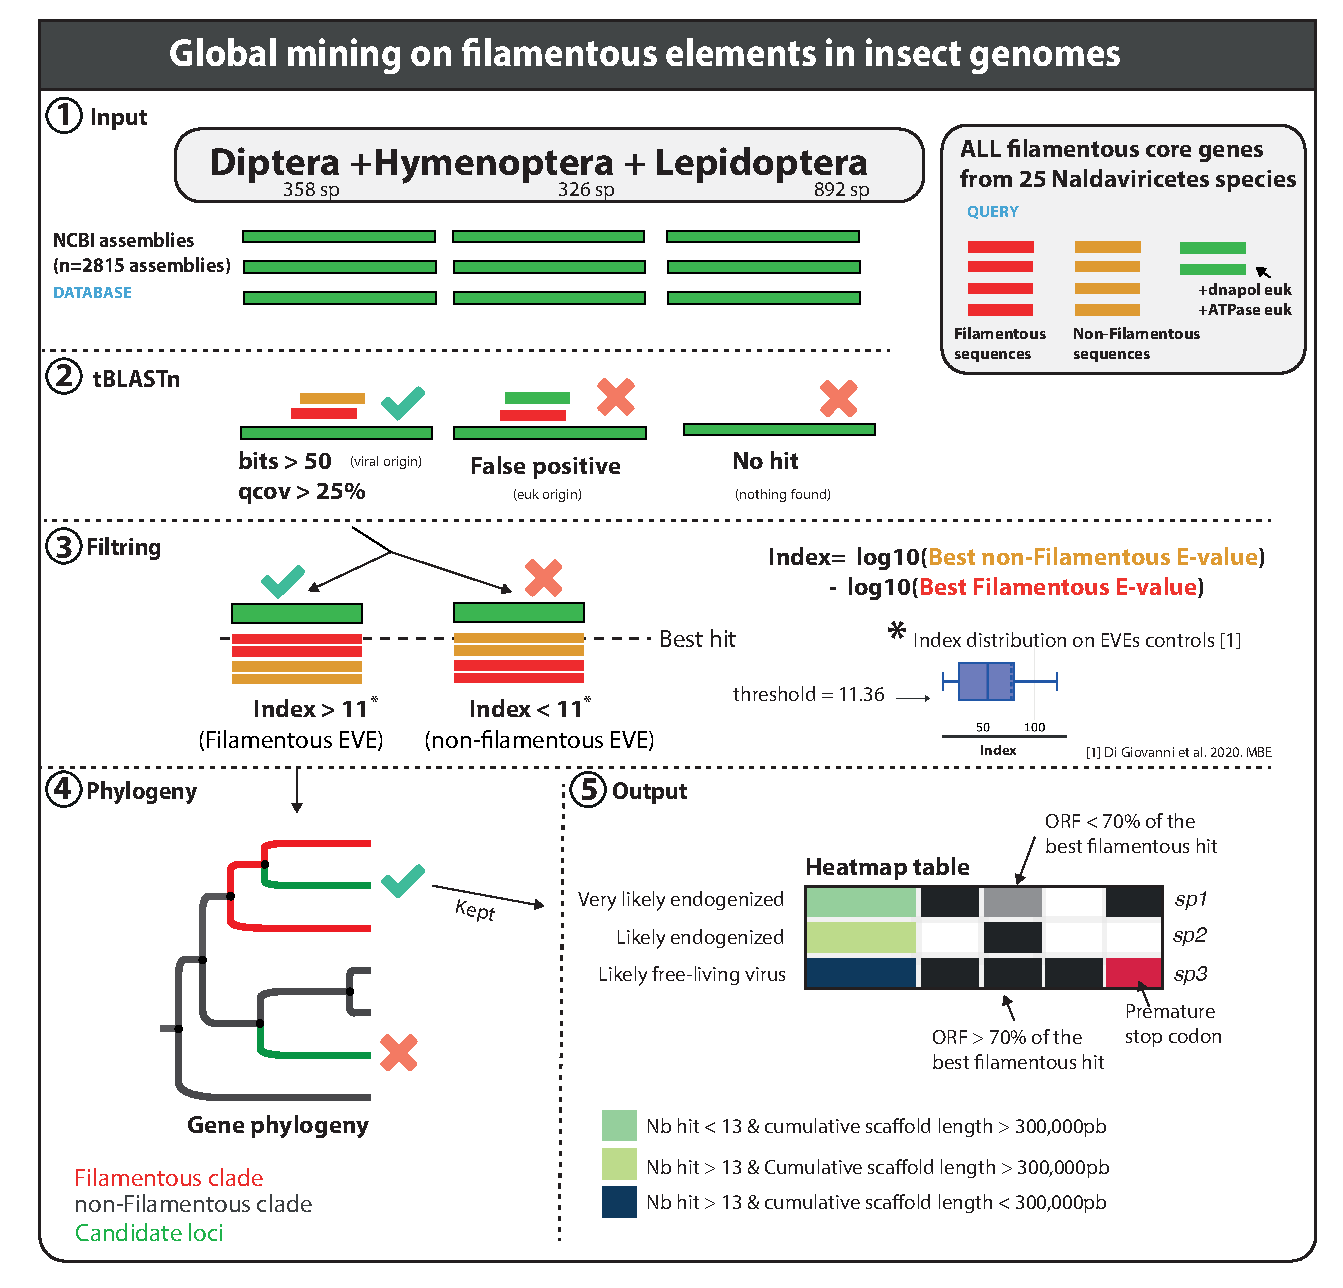
\includegraphics[width=\linewidth,height=\textheight,keepaspectratio]{PhD-master/figures/Pipeline_find_filamentous.pdf}\centering
\caption[Paper2:Graphical abstract of the pipeline to scan genomes for filamentous viruses]{\scriptsize\textbf{Graphical abstract summarizing the bioinformatics pipeline developed to search exhaustively for the presence of filamentous viral elements in Diptera, Hymenoptera and Lepidoptera assemblages.} The query corresponded to the set of the 29 core proteins detected in the genomes of the 25 \textit{Naldaviricetes} used in the main phylogeny (1). The database corresponded to all Hymenoptera, Diptera and Lepidoptera assemblies available in NCBI, BIPPA and a recent study (Bguinet et al., 2023, in review)(1). Only hits with a bit score greater than 40 and more than 25\% alignment coverage (to avoid identification of small domains homologies) were retained (2). We then compared the best alignment score of eukaryotic loci aligned with a filamentous protein to the best alignment score of a non-filamentous protein to filter out sequences by computing the difference of both log10 (e-value) scores (log10(e-value)virus-log10(e-value)euk). (3). To calibrate this score, we calculated its distribution from previously described cases of endogenization or free-living virus sequences in \textit{Leptopilina} species (Di Giovanni et al., 2020) and in the free-living species described in this paper. The minimum score from this distribution was then chosen as a minimal threshold to consider a hit as having a viral origin (3). For each candidate locus, we then built a phylogeny including the candidate locus and the 25 \textit{Naldaviricetes} sequences, in order to check whether manually the candidate locus was within an FV-like clade (4). Then we classified filamentous-like entities based on multiple metrics (5). Species with more than13 FV hits and a cumulative scaffold length greater 300,000bb was classified as “very likely endogenized”, species with more than 13 ORFs and a cumulative scaffold length greater than 300,000bp was classified as “likely endogenized”, and species with more than 13 ORFs and a cumulative scaffold length less than 300,000bp was classified as “likely free-living virus” since the size could correspond to the expected size for a FV virus (5).}
\label{figure:Pipeline_find_filamentous}
\end{figure}


\section{Suplementary figures}

\begin{figure}[!htpbt]
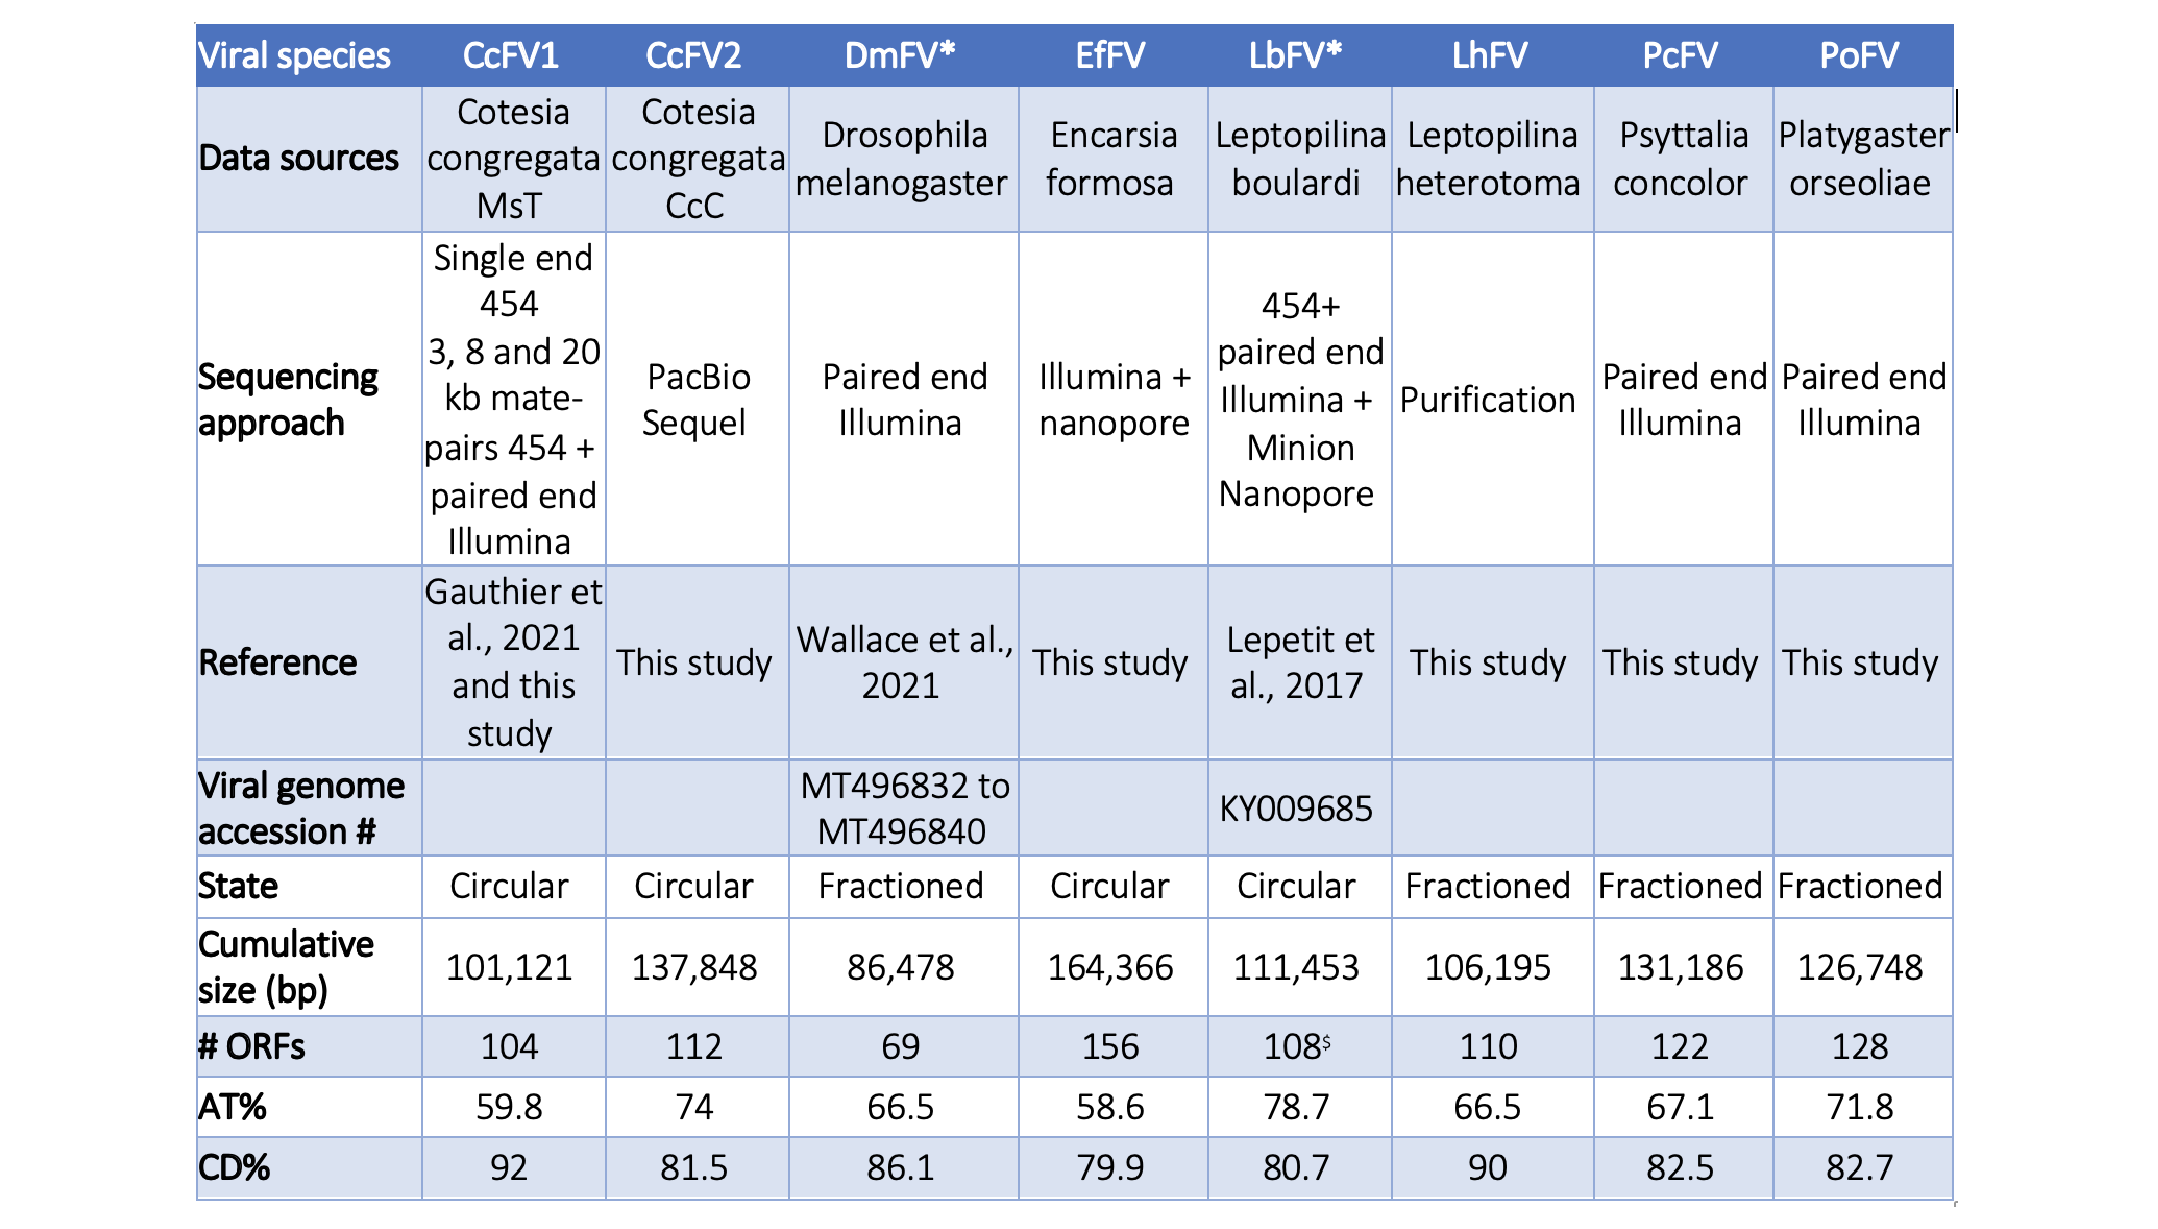
\includegraphics[width=\linewidth,height=\textheight,keepaspectratio]{PhD-master/figures/Table_genomes_filamentous.pdf}\centering
\caption[Paper2:Filamentous genomes informations]{\textbf{Table with all filamentous genome informations.} Stars means the genomes were previously published.}
\label{figure:Table_genomes_filamentous}
\end{figure}

\begin{figure}[!htpbt]
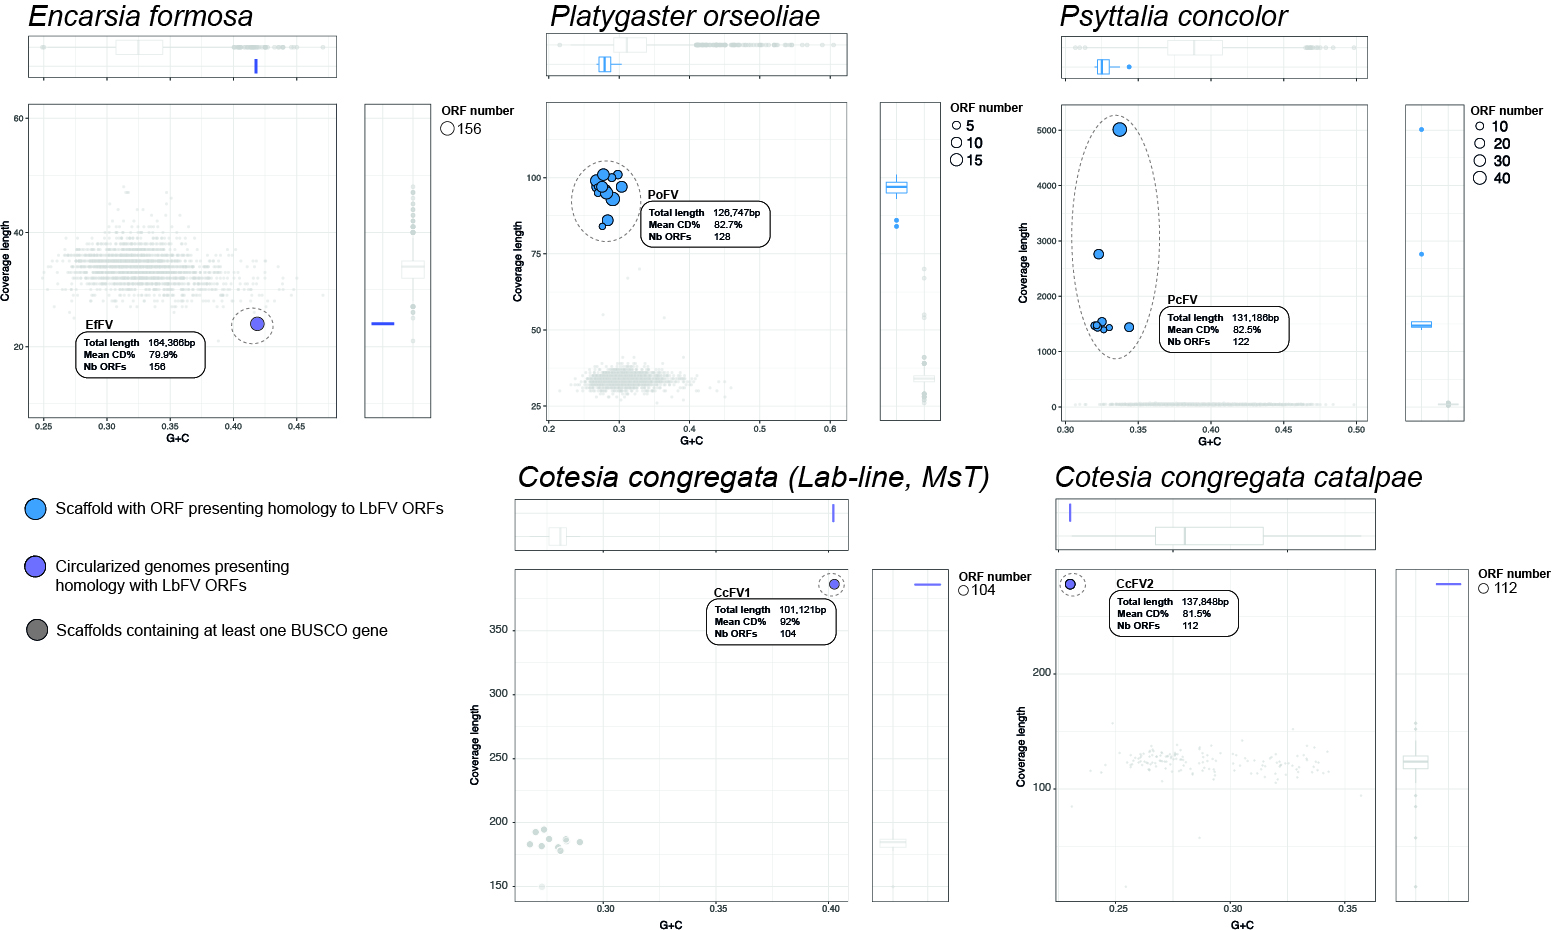
\includegraphics[width=\linewidth,height=\textheight,keepaspectratio]{PhD-master/figures/ALL_filamentous_cov_GC_plot.jpg}\centering
\caption[Paper2:Filamentous virus COV/GC content]{\textbf{G+C coverage distribution of scaffold containing homologies with filamentous ORFs.} Read mapping was done using illumina reads for EfFV, PoEFV and PcEFV, while 454 reads were used for CcFV1 and PacBio reads for CcFV2. The size of the dots corresponds to the number of ORFS predicted inside the scaffold. The color represents the genomic entity as follows (blue: scaffold presenting homologies with LbFV ORFs, purple = circularized genomes presenting homologies with LbFV ORFs, and grey = scaffold containing at least one BUSCO gene). The statistics in boxes correspond to statistics regarding the blue of purple circles. Total length il the sum of the bases, mean CD\% the mean coding density (ORF length / Total length), and Nb ORFs the number of predicted ORFs, respectively for all scaffolds/whole circularized genome for one viral species.}
\label{figure:ALL_filamentous_cov_GC_plot}
\end{figure}


\begin{landscape}
    
\begin{figure}[!htpbt]
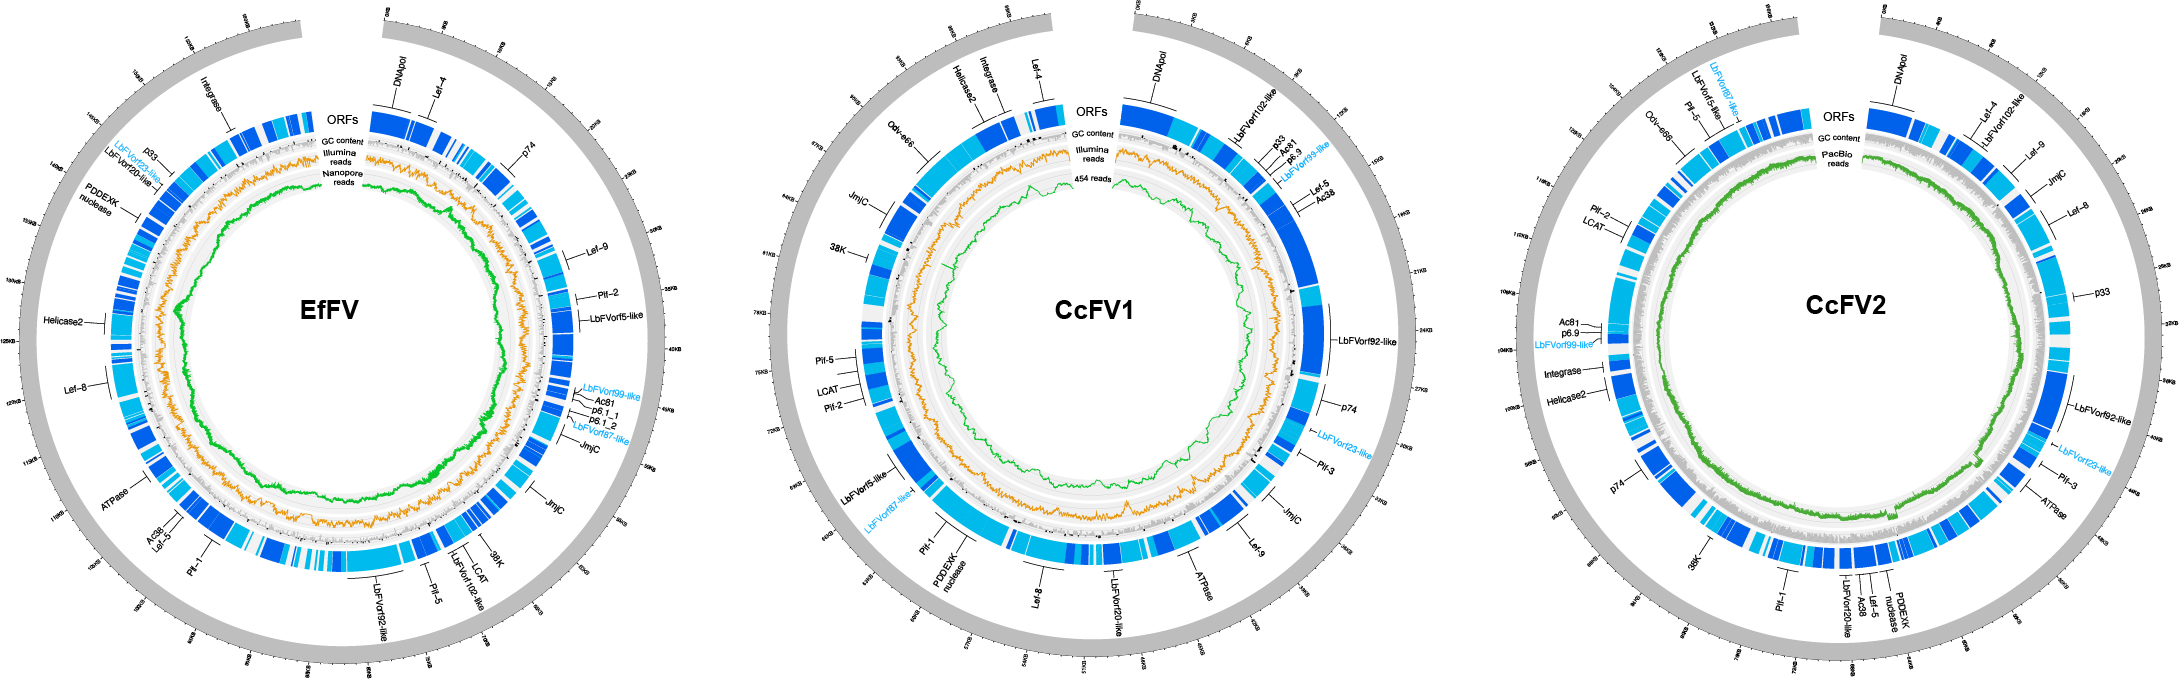
\includegraphics[width=\linewidth,height=\textheight,keepaspectratio]{PhD-master/figures/CcFV1_CcFV2_EfFV_circos.jpg}\centering
\caption[Paper2:Complete circularized filmentous genomes]{\textbf{Circular representation of the genomes of filamentous Encarsia formosa virus (EfFV), filamentous Cotesia congregata virus 1 (laboratory line) (CcFV1) and filamentous Cotesia congregata catalpae virus 2 (CcFV2)}. ORFs predicted using the comparison of Vgas (v2019) \citep{zhang_vgas_2019}, Prodigal (v2.6.3) \citep{hyatt_prodigal_2010} and Geneious(v 2019.2.3) \citep{kearse_geneious_2012} are displayed as blue rectangles where dark blue and light blue represent positive and negative strands respectively. The GC\% along the genome was calculated using the GC\_content.pl script written by Damien Richard (with a 100bp sliding window) and is displayed with bars where black bars represent GC\% $>$ 50\% and grey bars represent GC\% $<$ 50\%. The depth of coverage along the genomes was calculated using minimap2 (v 2.24-r1122) \citep{li_minimap2_2018} and samtools (v1.15) \citep{danecek_twelve_2021} and was extracted using Unipro UGENE (v43) \citep{okonechnikov_unipro_2012}. The two long read technologies (Oxford nanopore ONT, 454 and PacBio) are shown along the graph in green lines, and all Illumina paired-end reads are shown in orange lines. The figure was produced using the https://venyao.xyz/shinyCircos/ server.}
\label{figure:CcFV1_CcFV2_EfFV_circos}
\end{figure}

\end{landscape}

\begin{figure}[!htpbt]
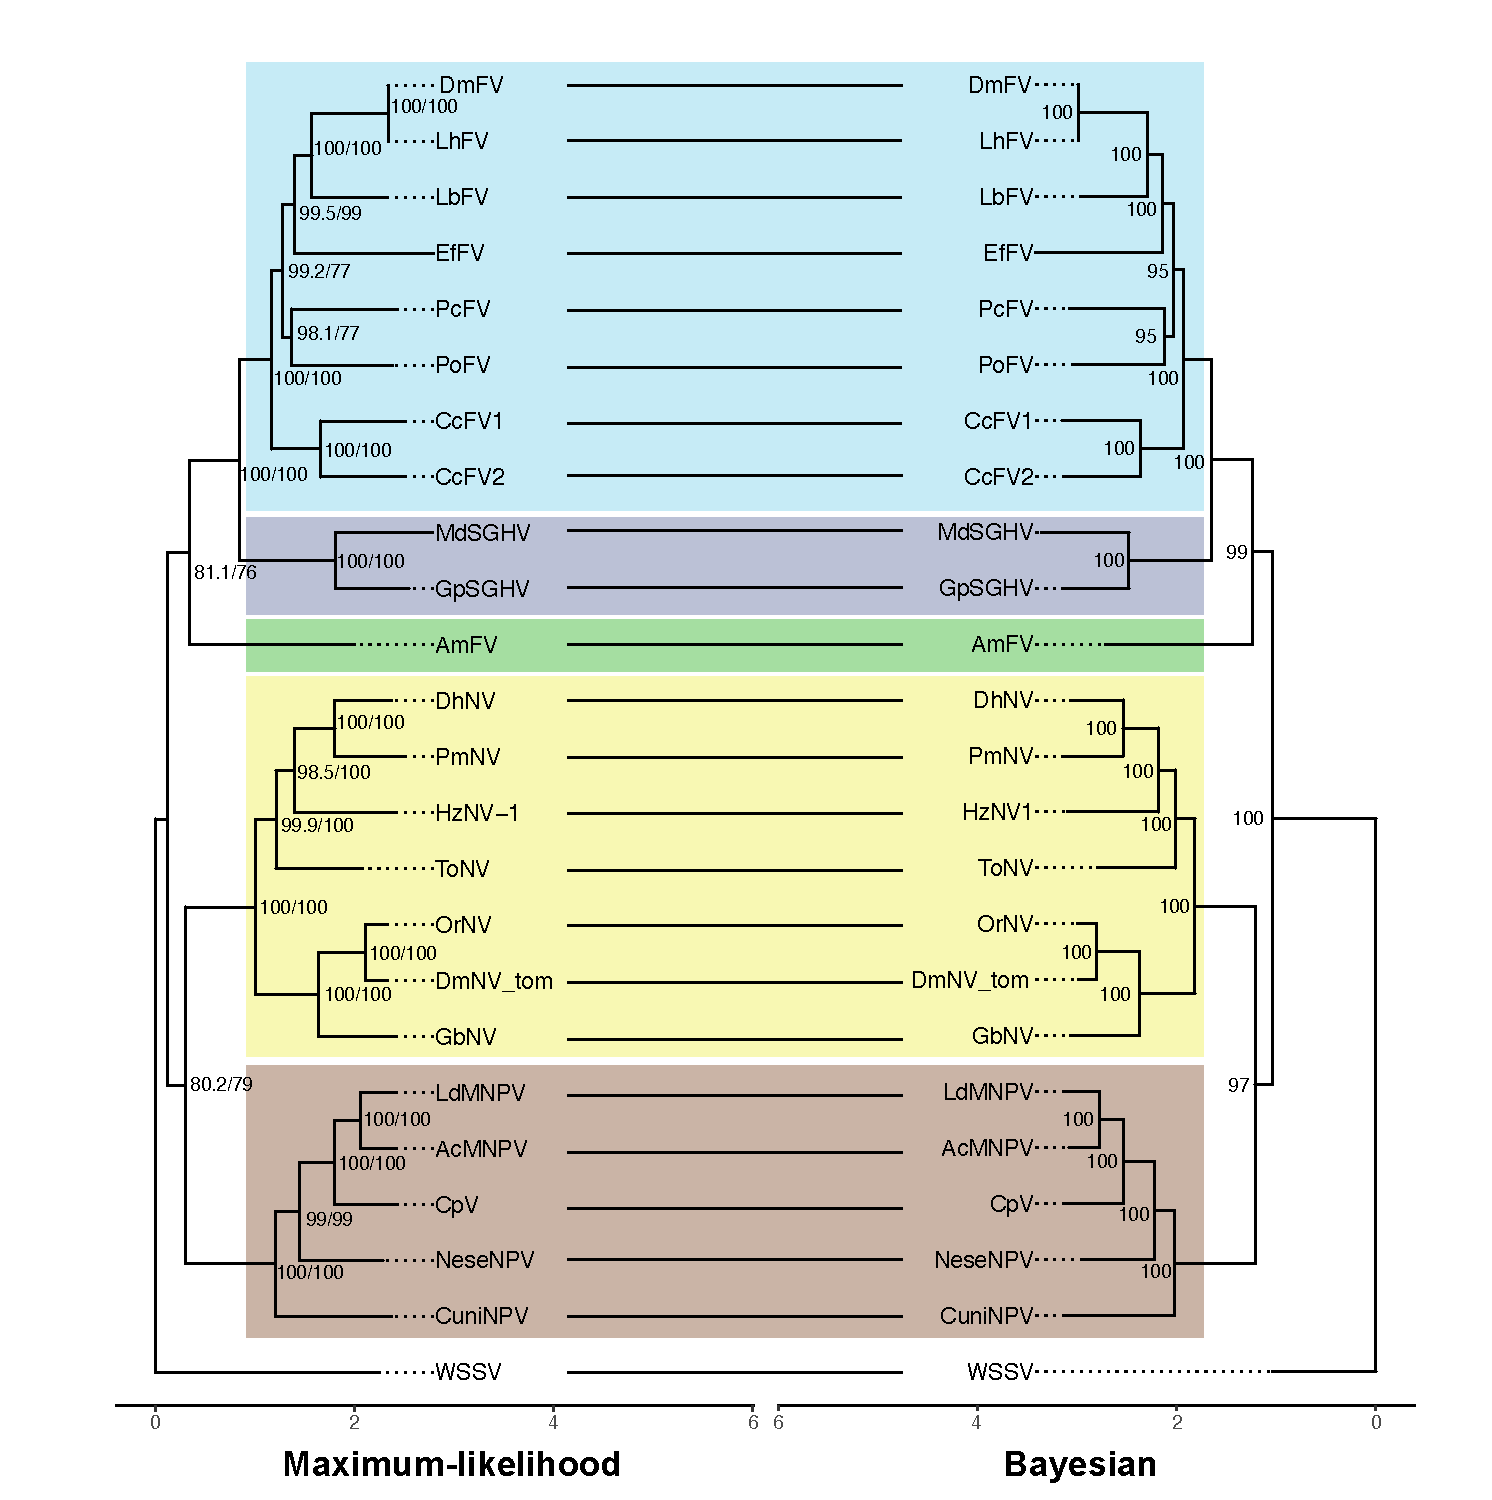
\includegraphics[width=\linewidth,height=\textheight,keepaspectratio]{PhD-master/figures/Bayesian_vs_ML_cophylogeny_filamentous.pdf}\centering
\caption[Paper2:dsDNA \textit{Naldaviricetes} phylogeny "core-genes method"]{\textbf{DsDNA viral phylogenetic trees inferred from gene clusters composed of all filamentous species.} Trees were inferred by Maximum likelihood (Iqtree) and Bayesian (MrBayes) methods using a partitioning amino-acid alignment and taking the \textit{Nimaviridae} species “WSSV” as outgroup. X-axis scale represents substitutions/site on both topologies. The colors refer to the dsDNA families (brown= Nudiviridae, yellow = Baculoviridae, Blue = FV-like family, purple= Hytrosaviridae, and green= AmFV-like family).}
\label{figure:Bayesian_vs_ML_cophylogeny_filamentous}
\end{figure}

\begin{figure}[!htpbt]
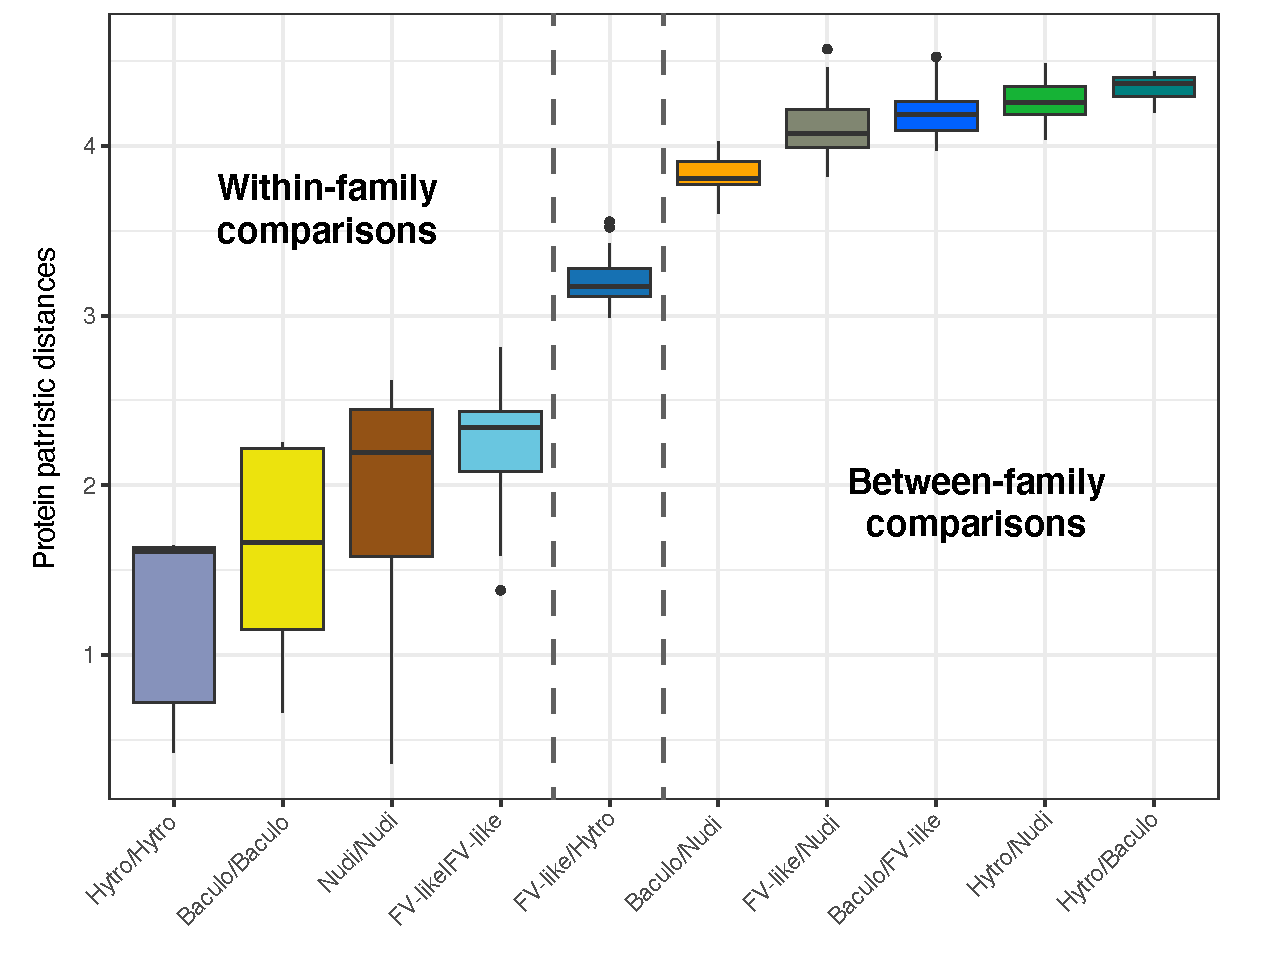
\includegraphics[width=\linewidth,height=\textheight,keepaspectratio]{PhD-master/figures/Patristic_distances_filamentous.pdf}\centering
\caption[Paper2:Patristic distance distributions between \textit{Naldaviricetes} viruses]{\textbf{Average patristic distance between species within the dsDNA virus phylogenetic clades.} The patristic distances were measured with the ape package v5.6 function cophenetic.phylo and correspond to the average number of protein substitutions per site between each species of a certain clade.}
\label{figure:Patristic_distances_filamentous}
\end{figure}

\begin{figure}[!htpbt]
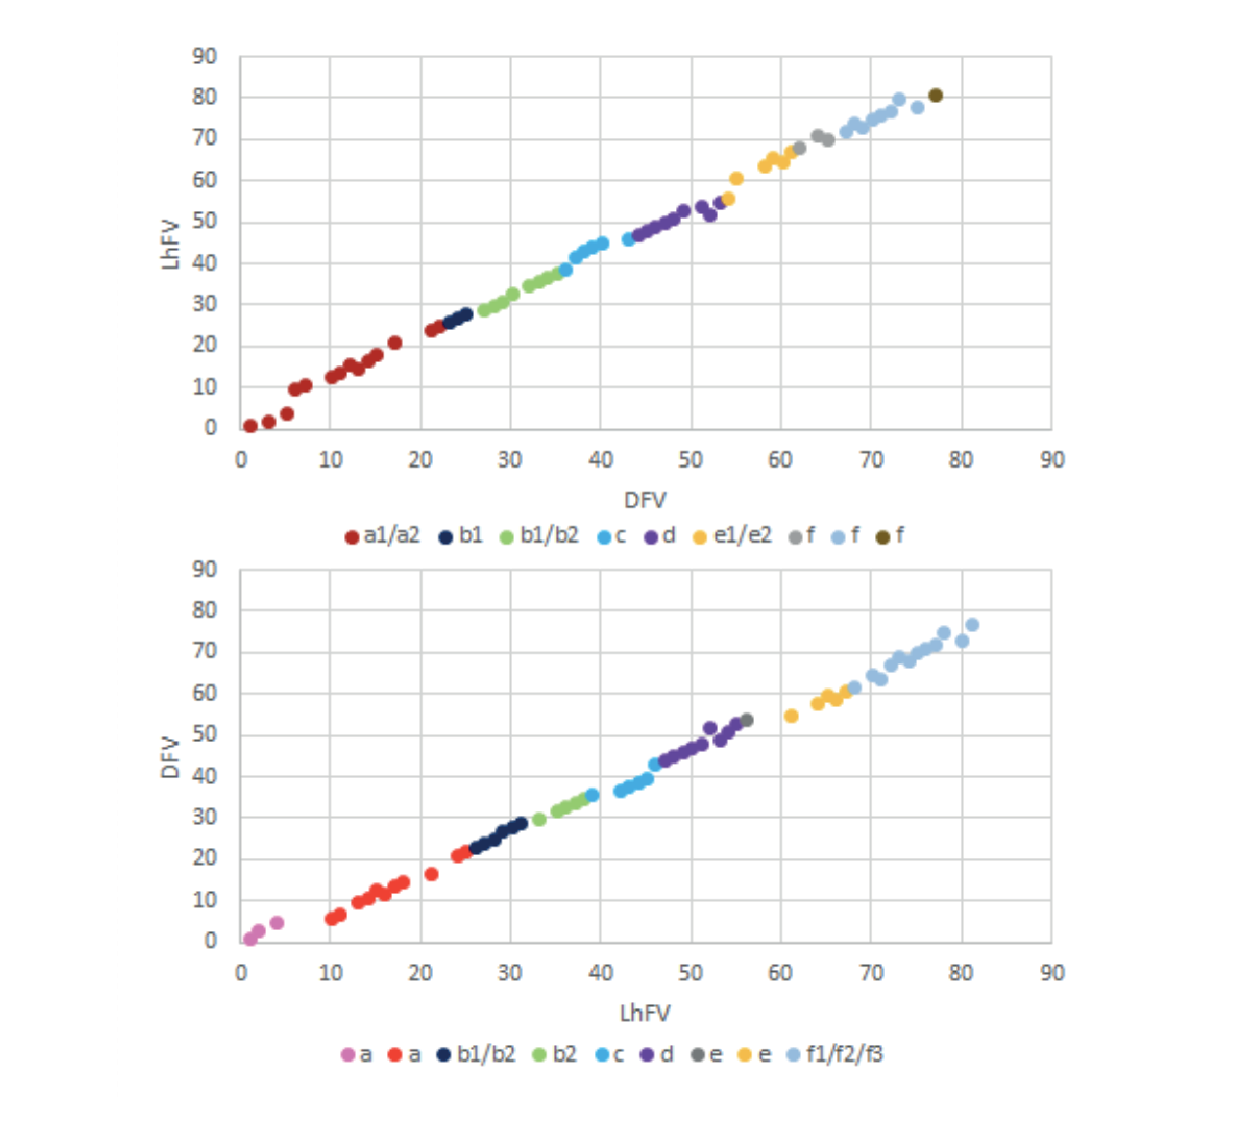
\includegraphics[width=\linewidth,height=\textheight,keepaspectratio]{PhD-master/figures/Syntenic_DmFV_LhFV.pdf}\centering
\caption[Paper2:Syntenic comparison between LhFV and DmFV]{\textbf{Gene parity plot comparisons of LbFV and DmFV}. The plots have been made with each of the two viruses as reference. The different colors associated with the letters refer to the different scaffolds of each genome. The plot using LhFV as reference allowed to merge the two scaffolds marked b1/b2 and the three scaffolds marked f1/f2/f3 of DmFV. Conversely, the plot using DmFV as a reference allows to merge the two scaffolds marked a1/a2, the two marked b1/b2 and e1/e2 of LhFV. The order of the scaffolds outside of the merged ones has been chosen arbitrarily.}
\label{figure:Syntenic_DmFV_LhFV}
\end{figure}

\begin{figure}[!htpbt]
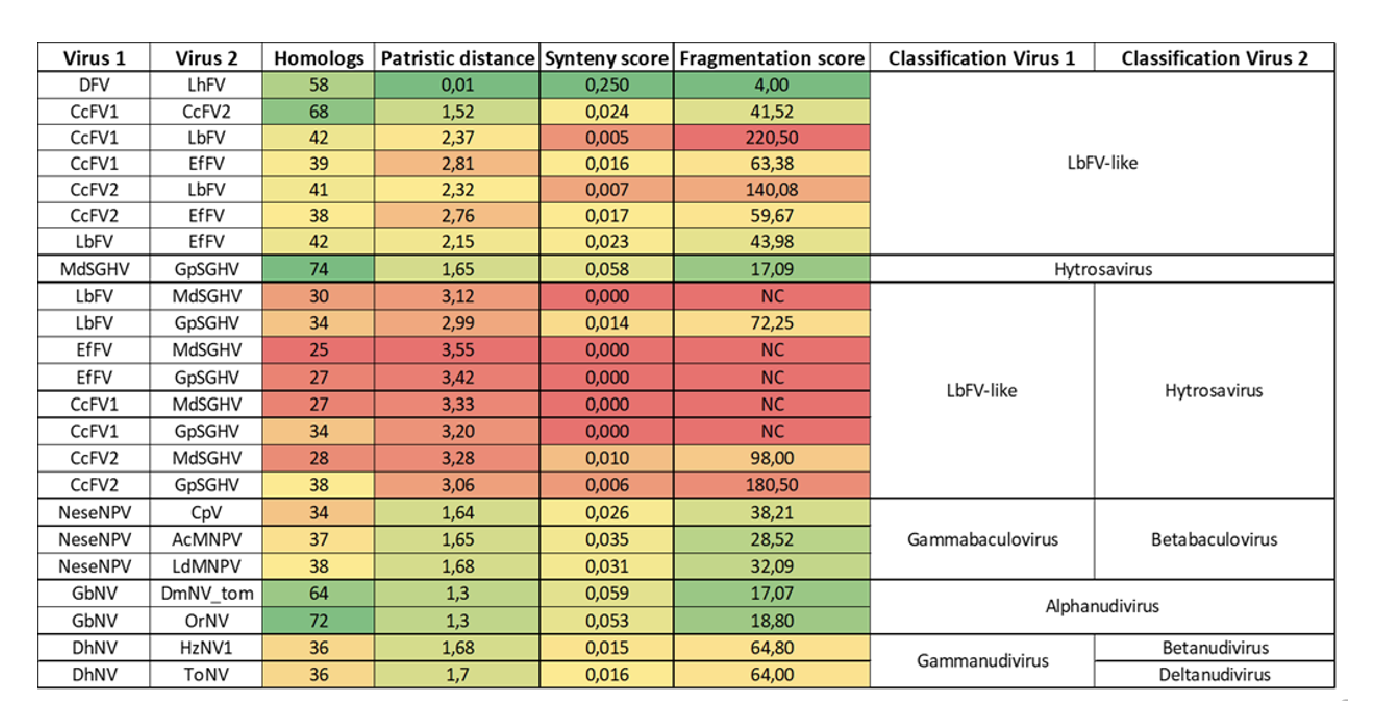
\includegraphics[width=\linewidth,height=\textheight,keepaspectratio]{PhD-master/figures/Syntenic_bloc_table.pdf}\centering
\caption[Paper2:Syntenic filamentous blocs]{\textbf{Table summarizing the results of collinearity analyses between the different viruses.} The colors from green to red indicate the level of similarity between two viruses}
\label{figure:Syntenic_bloc_table}
\end{figure}



\begin{figure}[!htpbt]
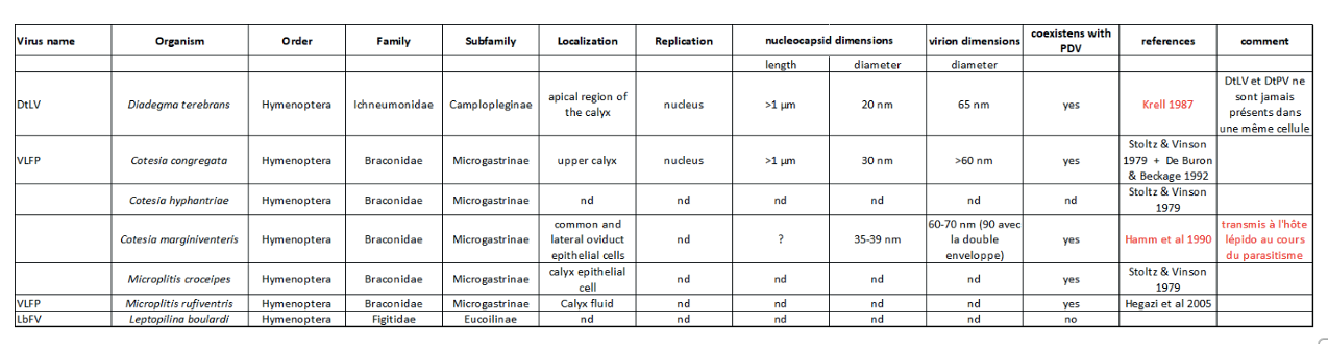
\includegraphics[width=\linewidth,height=\textheight,keepaspectratio]{PhD-master/figures/Table_filamentous_origins.pdf}\centering
\caption[Paper2:Filamentous description in literature]{\textbf{Occurence of filamentous viruses described transmission electron microscopy in the litterature}.}
\label{figure:Table_filamentous_origins}
\end{figure}

